% Modified from AAAS Science LATEX template
% Use only LaTeX2e, calling the article.cls class and 12-point type.

\documentclass[10pt, oneside]{article}

\usepackage{helvet}
\renewcommand{\familydefault}{\sfdefault}
\usepackage{graphicx}
\usepackage{caption}
\usepackage{float}
\captionsetup{font=small}
\usepackage{textcomp}
\usepackage{url}
\usepackage{cite}
\usepackage{nameref}
\usepackage[none]{hyphenat}%%%%
\usepackage[utf8]{inputenc}
\usepackage[english]{babel}
\usepackage[T1]{fontenc}
\usepackage{multicol}
\setlength{\columnsep}{0.5cm}
\usepackage{titlesec}

\titleformat*{\section}{\large\bfseries}
\titleformat*{\subsection}{\normalsize\bfseries}
\titleformat*{\subsubsection}{\normalsize\bfseries}

% Page setup
\topmargin -2cm
\oddsidemargin -1cm
\evensidemargin 1cm
\textwidth 18cm
\textheight 24cm
\footskip 1.0cm


\newcommand{\beginsupplement}{%
  \setcounter{table}{0}
  \renewcommand{\thetable}{S\arabic{table}}%
  \setcounter{figure}{0}
  \renewcommand{\thefigure}{S\arabic{figure}}%
}

% Include the date command, but leave its argument blank to prevent date print.
\date{}

%%%%%%%%%%%%%%%%% END OF PREAMBLE %%%%%%%%%%%%%%%%

% Initialize use of code blocks with syntax highlighting
\usepackage{listings}
\usepackage{color}

\definecolor{dkgreen}{rgb}{0,0.6,0}
\definecolor{gray}{rgb}{0.5,0.5,0.5}
\definecolor{mauve}{rgb}{0.58,0,0.82}

\lstset{frame=tb,
  language=Java,
  aboveskip=3mm,
  belowskip=3mm,
  showstringspaces=false,
  columns=flexible,
  basicstyle={\small\ttfamily},
  numbers=none,
  numberstyle=\tiny\color{gray},
  keywordstyle=\color{blue},
  commentstyle=\color{dkgreen},
  stringstyle=\color{mauve},
  breaklines=true,
  breakatwhitespace=true,
  tabsize=3
}

%%%%%%%%%%%%%%%%% START OF DOCUMENT %%%%%%%%%%%%%%%%

\begin{document}

% Double-space the manuscript.
\baselineskip24pt

% Paper title
\noindent
{\huge
\textbf{XPRESSyourself: Enhancing, Standardizing, and \\
Automating Ribosome Profiling Computational \\
Analyses Yields Improved Insight into Data
}
}

\bigskip

%\noindent
%{\large
%\textit{Short Title: XPRESSyourself: Enhanced Ribosome Profiling Analysis Improves Data Insight}
%} \\


% Author info

% Author list/order:
\noindent
{\large
\textbf{Jordan A. Berg,$^{1\ast}$ Jonathan R. Belyeu,$^{2}$ Jeffrey T. Morgan,$^{1}$ Yeyun Ouyang,$^{1}$ Alex J. Bott,$^{1}$ Aaron R. Quinlan,$^{2,4,5}$ Jason Gertz,$^{3}$ Jared Rutter$^{1,6\ast}$
}
} \\

\noindent
{$^{1}$Department of Biochemistry, University of Utah, Salt Lake City, UT, USA, 84112.}\\
{$^{2}$Department of Human Genetics, University of Utah, Salt Lake City, UT, USA, 84112.}\\
{$^{3}$Department of Oncological Sciences, University of Utah, Salt Lake City, UT, USA, 84112.}\\
{$^{4}$USTAR Center for Genetic Discovery, University of Utah, Salt Lake City, UT, USA, 84112.}\\
{$^{5}$Department of Biomedical Informatics, University of Utah, Salt Lake City, UT, USA, 84112.}\\
{$^{6}$Howard Hughes Medical Institute, University of Utah, Salt Lake City, UT, USA, 84112.}\\
{$^\ast$Address correspondence to: jordan.berg@biochem.utah.edu, rutter@biochem.utah.edu}

\pagebreak

% Abstract
\section*{Abstract}
\noindent
Ribosome profiling, an application of nucleic acid sequencing for monitoring ribosome activity, has revolutionized our understanding of protein translation dynamics. This technique has been available for a decade, yet the current state of publicly available computational tools for these data is bleak. We introduce XPRESSyourself, an analytical toolkit that eliminates barriers and bottlenecks associated with this specialized data type by filling gaps in the computational toolset for both experts and non-experts of ribosome profiling. XPRESSyourself automates and standardizes analysis procedures, decreasing time-to-discovery and increasing reproducibility. This toolkit acts as a reference implementation of current best practices in ribosome profiling analysis. We demonstrate this toolkit's \\performance on publicly available ribosome profiling data and associated bulk RNA-Seq data by rapidly identifying hypothetical mechanisms related to neurodegenerative phenotypes and neuroprotective mechanisms of the \\small-molecule ISRIB during acute cellular stress. XPRESSyourself brings robust, rapid analysis of ribosome-profiling data to a broad and ever-expanding audience and will lead to more reproducible and accessible measurements of translation regulation. The XPRESSyourself software is perpetually open-source under the GPL-3.0 license and is hosted at https://github.com/XPRESSyourself, where the user can find additional documentation and report issues.\\

%\section*{Author Summary}
%\noindent
%Ribosome profiling allows scientists to explore the process of how proteins, the building blocks of life, are created and regulated. However, computational methods for analyzing this data type are incomplete. We developed \\XPRESSyourself, a software suite that fills these gaps in available tools for ribosome profiling analysis. This toolkit additionally serves as a reference implementation of current best practices in ribosome profiling analysis to aid users in processing their data correctly. Using this toolkit and pipeline, we processed publicly available ribosome profiling data and were able to discover potential mechanisms of how neurodegeneration occurs during acute neurological trauma.\\

\setlength{\parindent}{2em}

\section*{Introduction}
High-throughput sequencing data has revolutionized biomedical and biological research. One such application of this consequential technology is ribosome profiling, which, coupled with bulk RNA-Seq, measures translation efficiency, translation pausing, novel protein translation products, and more. \cite{ingolia_science, riboseq_overview, ingolia_meth}. Though ribosome profiling has matured, there remains an abundance of biases and peculiarities associated with each analytical method or tool, which are often obscured to a user \cite{gerashchenko_nar, analysis_biases, riboseq_biases, riboseq_biases2, riboseq_biases3}. Additionally, standardized methods for handling this unique data type remain elusive. This has been problematic and evidenced by various studies using vague or opaque methods for data analysis (for several examples, see \cite{isrib_riboseq, scripts_1, scripts_2, scripts_3, scripts_4}), or methods rely on outdated tools, such as Bowtie \cite{bowtie}, which continues to be used in various ribosome profiling studies for alignment. In this example, this tool is inappropriate as it is unable to map reads across splice junctions \cite{analysis_biases}. Very few labs have the tools to separate the biological signals in ribosome profiling data from inherent biases of the experimental measurements, and these tools are not readily accessible by the community. This is a critical time in the rapidly expanding influence of ribosome-footprint profiling. For too long, the bioinformatic know-how of this incredibly powerful technique has been limited to a small handful of labs. As more and more ribosome profiling studies are performed, more and more labs will lack the ability to analyze their data with ease and fidelity. Few if any extant pipelines or toolkits offer a thorough set of integrated tools for assessing standard quality control metrics or performing proper reference curation and reducing systematic biases across any organism, particularly with ribosome profiling data \cite{galaxy, ribogalaxy, nextflow_pipeline, dnanexus_pipeline, riboviz}.\par

For example, one issue in ribosome profiling is the pile-up of ribosomes at the $5'$- and $3'$- ends of coding regions within a transcript is a systematic biological signal arising from the slower kinetics of ribosome initiation and termination compared to translation elongation and is often not relevant to measurements of translation regulation \cite{gerashchenko_nar, artieri_gr, hussman_plosg}. These pile-ups can dramatically skew ribosome footprint quantification and measurements of translational efficiency. Leaders in the field currently recommend excluding these pile-up-prone regions when quantifying ribosome profiling alignments \cite{ingolia_meth, weinberg_reports}; however, no publicly available computational tools currently exist to facilitate these automated adjustments to reference transcripts. Curating references for this ability requires advanced implementations to achieve correctly and robustly. In addition, downstream data visualization methods presently available are not optimized to analyze and compare translationally regulation regions of a gene. \par

To address these deficiencies in the public ribosome profiling computational toolkit, we developed \\XPRESSyourself, a computational toolkit and server-less, adaptable pipeline that bridges these and other gaps in ribosome profiling data analysis. XPRESSyourself implements the complete suite of tools necessary for ribosome profiling and bulk RNA-Seq analysis in a robust and easy-to-use software package, often packaging tasks that would typically require hundreds to thousands of lines of code into a single command. This software will lead to more reproducible and more accessible measurements of translation regulation. For instance, XPRESSyourself creates the mRNA annotation files necessary to remove confounding systematic factors during quantification and analysis of ribosome profiling data to measure translation accurately. It also provides a built-in capacity to quantify and visualize differential upstream open-reading frame (uORF) usage by generating IGV-like, intron-less plots for easier visualization \cite{igv}. The ability to visualize (and in another XPRESSyourself module, quantify) the usage of micro-uORFs is important in exploring regulatory events or mechanisms in a wide array of biological responses and diseases. XPRESSyourself also introduces a tool for efficient identification of the most problematic rRNA fragments for targeted depletion, which provides immense financial and experimental benefits to the user as ribosome footprint signal can be better amplified over rRNA noise. Tools like this will become vital as ribosome profiling moves into development in new organisms.\par

XPRESSyourself aims to address the lack of consensus in analytical approaches used to process ribosome profiling data by acting as a reference implementation of current best practices for ribosome profiling analysis. While a basic bioinformatic understanding is becoming more commonplace amongst the scientific community, the intricacies of processing RNA-Seq data remain challenging for many. Moreover, many users are often not aware of the most up-to-date tools or the appropriate settings for their application \cite{costello_npjsba, funari_science}. Even for the experienced user, developing robust automated pipelines that accurately process and assess the quality of these datasets can be laborious. The variability that inevitably arises with each lab or core facility designing and using distinct pipelines is also a challenge to reproducibility in the field. XPRESSyourself curates the state-of-the-art methods for use and where a required functionality is unavailable, introduces a thoroughly tested module to fill that gap. In addition to the new tools described above, the toolkit provides the user with a complete suite of software to handle pre-processing, aligning, and quantifying of sequence reads, performing quality control via various meta-analyses of pre- and post-processed reads, in many cases tailored for ribosome profiling but flexible enough to handle general RNA-Seq datasets. While some of these steps may be considered more mundane, we eliminate the need of each user to rewrite even simple functionality and promote reproducibility between implementations. To aid users of any skill-level in using this toolkit, we provide thorough documentation, walkthrough videos, and interactive command builders to make usage as easy as possible, while allowing for broad use of this toolkit on high-performance clusters.\par

Finally, the most broadly relevant aspect of our update and streamlining of ribosome-profiling analysis is the novel biological insights we are able to obtain from published datasets. We highlight this in the ISRIB ribosome-profiling study discussed in this manuscript, where we are able to observe significant translation regulation that was missed previously when the data were initially analyzed using now outdated techniques. This analysis generates novel hypotheses for genes potentially involved in neurodegeneration in humans, but more broadly emphasizes the benefit of analysis and re-analysis of data using the complete and up-to-date benchmarked methodology provided within XPRESSyourself.\\

\section*{Design and Implementation}
\subsection*{Architecture and Organization}
XPRESSyourself is currently partitioned into two software packages, XPRESSpipe and XPRESSplot. XPRESSpipe contains automated pipelines tailored for ribosome profiling, single-end RNA-Seq, and paired-end RNA-Seq datasets. Figure \ref{fig:outputs} outlines tasks completed within the pipelines. Individual sub-modules can be run automatically through a pipeline or manually step-by-step. Modules optimize available computational resources to deliver results as quickly as possible. XPRESSplot is available as a Python library and provides an array of analytical methods specifically for sequence data, but tractable to other data types. For a comparison of how XPRESSyourself compares to other available software packages available at time of writing, we refer the reader to Figure \ref{fig:supplement1} \cite{galaxy, ribogalaxy, pausepred, anota2seq, riboprofiling, riborex, mqc, shoelaces, supertranscripts, systempiper, orfik, comet_1, comet_2, riboseqr, deeptools, picard, rose, rust, xtail, ribodiff, ribotaper, ribomap_1, ribomap_2, plastid, riboviz, ribostreamr, scikit_ribo, spectre}.\par

XPRESSyourself aims to make ribosome profiling and sequence analysis as easy and accessible as possible to all users. As such, an integrated command builder for reference curation and sample analysis can be run by executing \texttt{xpresspipe build}. This command builder will walk the user through potential considerations based on their library preparation method and build the appropriate command for execution on their personal computer or a supercomputing cluster.\par

The software is designed such that updating and testing of a new module, or updating dependency usage, are facile tasks for a trained bioinformatician. More details on current and future capabilities can be found in each package's documentation \cite{xpresspipe_docs, xpressplot_docs} or their respective \texttt{versions} page on their respective repository pages \cite{xpressyourself}.\\

\begin{figure*}
\centering
  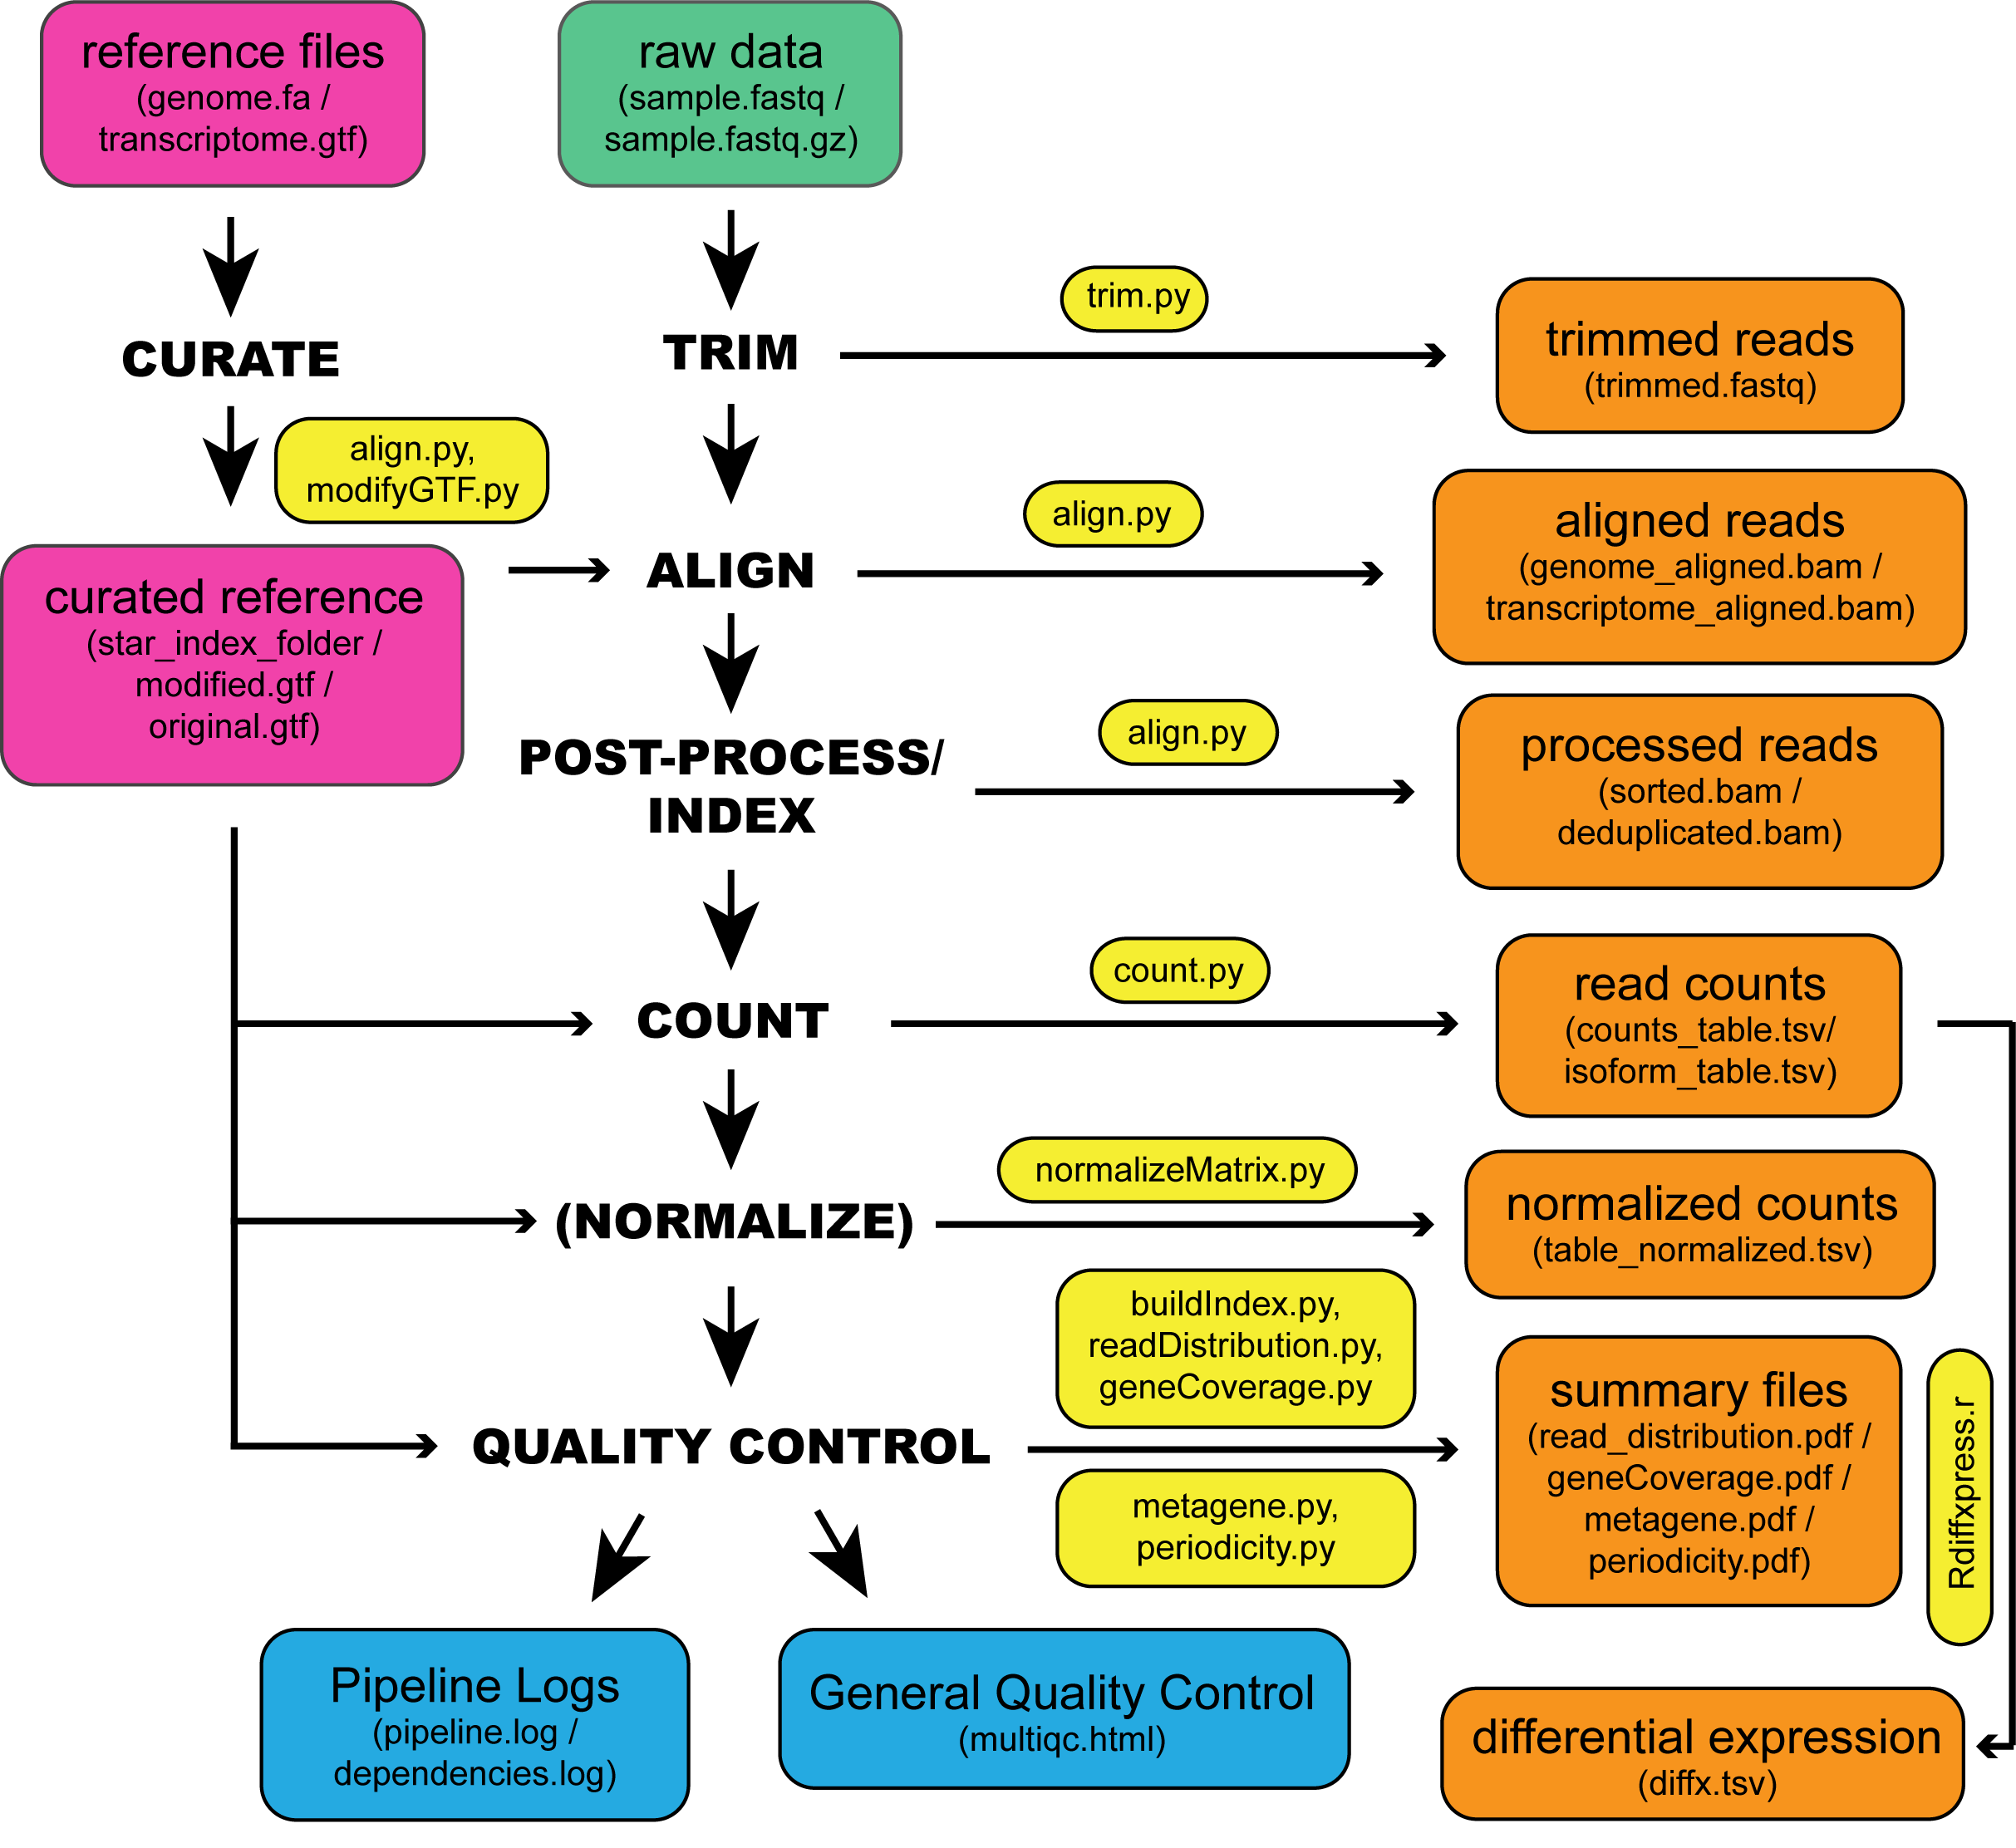
\includegraphics[width=160mm]{figures/xpresspipe_figure1.png}
  \caption{\textbf{Workflow schematic of the inputs, outputs, and organization of XPRESSpipe.} Representation of the general steps performed by XPRESSpipe with data and log outputs. Steps in parentheses are optional to the user. Input and output file types are in parentheses for each input or output block. Main script(s) used for a given step are in yellow blocks. The green block indicates input sequence file(s). Pink blocks indicate reference input files and curated reference. Orange blocks indicate output files. Blue blocks indicate general quality control and log file outputs.}
  \label{fig:outputs}
\end{figure*}

\subsection*{Automated Reference Curation}
The first step of RNA-Seq alignment is curating an organism reference to which the alignment software will map sequence reads. XPRESSpipe uses STAR \cite{star} for mapping reads as it has been shown consistently to be the best performing read aligner for RNA-Seq data \cite{alignment_benchmark, alignment_benchmark2}. The appropriate reference files are automatically curated by providing the appropriate GTF file saved as \texttt{transcripts.gtf} and the directory path to the genomic FASTA file(s). Additional modifications to the GTF file required for ribosome profiling or desired for RNA-Seq are discussed in the next section.\\

\subsection*{GTF Modification}
For ribosome profiling, frequent read pile-ups are observed at the $5'$- and $3'$- ends of an open reading frame which are largely uninformative as to the translational efficiency of the gene \cite{gerashchenko_nar}. While these pile-ups can be indicative of true translation dynamics \cite{tuller_alt}, more recently leaders in the field have determined that these regions should be ignored when quantifying reads and calculating translation efficiency \cite{ingolia_meth, weinberg_reports}. By providing the \texttt{-{}-truncate} argument during reference curation, the $5'$- and $3'$- ends of each coding region will be recursively trimmed until the specified amounts are removed from coding space. A recursive strategy is required here as GTF file formats section out each CDS region on each exon as separate records. By default, 45 nt will be trimmed from the $5'$- ends and 15 nt from the $3'$-ends, as is the convention within the ribosome profiling field \cite{ingolia_meth}, but these amounts can be modified. The resulting output file should be used to process ribosome footprint libraries, along with their corresponding bulk RNA-Seq libraries. If generating a GTF file for use solely with general bulk RNA-Seq datasets, this file should not be truncated.\par

Additionally, parameters that can be provided during this step to retain only protein-coding genes records. As ribosomal RNAs and other non-coding RNAs can be highly abundant in RNA-Seq experiments, it is often recommended to not include these sequences for quantification. This acts as a read masking step to exclude non-protein coding transcripts from downstream analyses. Parameters can also be provided to retain only the Ensembl canonical transcript record. This can be useful for some tools that penalize reads that overlap multiple isoforms of the same gene. If using HTSeq with default XPRESSpipe parameters or Cufflinks to quantify reads, this is not necessary as they do not penalize a read mapping to multiple isoforms of the same gene or are capable of handling quantification of different isoforms of a gene \cite{htseq, cufflinks}.\\

\subsection*{Read Processing}
\textbf{Pre-Processing}. In order for sequence reads to be mapped to the genome, reads generally need to be cleaned of artifacts from library creation. These include adaptors, unique molecular identifier (UMI) sequences, and technical errors in the form of low-quality base calls. Parameters, like minimum acceptable quality or length, can be modified, or features such as UMIs can be specified to identify and group PCR artifacts for later removal \cite{umi, umitools}.\par

\noindent\textbf{Mapping}. Reads are aligned to the reference genome with STAR, which, despite being more memory-intensive, is one of the fastest and most accurate sequence alignment options currently available \cite{star, alignment_benchmark, alignment_benchmark2}. XPRESSpipe is capable of performing a single-pass, splice-aware, GTF-guided alignment or a two-pass alignment of reads wherein novel splice junctions are determined and built into the reference, followed by alignment of reads to the new reference. A coordinate-sorted and indexed BAM file is output by STAR. We abstain from rRNA negative alignment at this step as downstream analysis of these mapped reads could be of interest to some users. When rRNA alignment is preferred, a protein-coding-only GTF file should be provided during quantification. \par

\noindent\textbf{Quantification}. XPRESSpipe further processes alignment files by optionally parsing for unique alignments for downstream analyses. PCR duplicates are also detected and marked or removed for downstream analyses; however, these files are only used for relevant downstream steps or if the user specifies to use these de-duplicated files in all downstream steps. Use of de-duplicated alignment files may be advisable in situations where the library complexity profiles (discussed below) exhibit high duplication frequencies. However, generally the abundance of PCR-duplicates is low in properly-prepared sequencing libraries; thus, doing so may be overly stringent and unnecessary \cite{umi}. Optionally, BED coverage files can also be output.\par

\noindent\textbf{Post-Processing}. XPRESSpipe quantifies read alignments for each input file using HTSeq with the \\\texttt{intersection-nonempty} method by default \cite{htseq, count_benchmark}. We use this quantification method as it conforms to the current TCGA processing standards and is favorable ion the majority of applications \cite{tcga}. If masking of non-coding RNAs is desired, a \texttt{protein\_coding} modified GTF file should be provided for the \texttt{-{}-gtf} argument. HTSeq is recommended for processing ribosome profiling data as it allows selection of feature type across which to quantify, thus allowing for quantification across the CDSs of a transcript instead of entire exons. If a user is interested in quantifying ribosome occupancy of transcript uORFs in ribosome footprint samples, they can provide \texttt{five\_prime\_utr} or \texttt{three\_prime\_utr} for the \texttt{-{}-feature\_type} parameter if such annotations exist in the organism of interest's GTF file. If the user is interested in isoform abundance estimation, Cufflinks is alternatively available for quantification \cite{cufflinks, count_benchmark}. If Cufflinks is provided for a ribosome profiling dataset, XPRESSpipe will use Ribomap to provide isoform abundance of ribosome profiles \cite{ribomap_1, ribomap_2}.\par

\noindent\textbf{Normalization}. Methods for count normalization are available within XPRESSpipe by way of the XPRESSplot package. For normalizations correcting for transcript length, the appropriate GTF must be provided. Sample normalization methods available include reads-per-million (RPM), Reads-per-kilobase-million (RPKM) or \\Fragments-per-kilobase-million (FPKM), and transcripts per million (TPM) normalization \cite{evans_briefbio}. For samples sequenced on different flow cells, prepared by different individuals, or on different days, the \texttt{-{}-batch} argument should be provided along with the appropriate metadata matrix \cite{sva}.\\

\subsection*{Quality Control}
\textbf{Read Length Distribution}. The lengths of all reads are analyzed after trimming. By assessing the read distribution of each sample, the user can ensure the expected read size was sequenced. This is particularly helpful in ribosome profiling experiments for verifying the requisite 17-33 nt ribosome footprints were selectively captured during library preparation \cite{ingolia_meth, fp_range}. Metrics here, as in all other quality control sub-modules, are compiled into summary figures for easy experiment-wide assessment by the user. \par

\noindent\textbf{Library Complexity}. Measuring library complexity is an effective method for analyzing the robustness of a sequencing experiment in capturing various, unique RNA species. As the majority of RNA-Seq preparation methods involve a PCR step, sometimes particular fragments will be favored and over-amplified in contrast to others. By plotting the number of PCR replicates versus expression level for each gene, one can monitor any effects of limited transcript capture diversity and/or high estimated PCR duplication rate on the robustness of their libraries. This analysis is performed using dupRadar \cite{dupradar} where inputs are PCR duplicate-tagged BAM files output during post-processing. Metrics are then compiled and plotted by XPRESSpipe.\par

\noindent\textbf{Metagene Estimation Profile}. To identify any general biases for the preferential capture of the $5'$- or $3'$- ends of transcripts, metagene profiles are generated for each sample. This is performed by determining the meta-genomic coordinate for each aligned read in exon space. Coverage is calculated for each transcript, normalized, and combined to eliminate greediness of super-expressors in profile coverage. Required inputs are an indexed BAM file and an un-modified GTF reference file. Outputs include metagene metrics, individual plots, and summary plots.\par

\noindent\textbf{Gene Coverage Profile}. Extending the metagene estimation analysis, the user can focus on the coverage profile across a single gene. Although traditional tools like IGV \cite{igv} offer the ability to perform such tasks, XPRESSpipe offers the ability to collapse the introns to observe coverage over exon space only. This is helpful in situations where massive introns spread out exons and make it difficult to visualize exon coverage for the entire transcript in a concise manner. CDS region is identified to aid ribosome profiling data users in identifying CDS coverage and uORF translation events. When running an XPRESSpipe pipeline, a housekeeping gene will be processed and output for the user's reference. Figure \ref{fig:supplement2} provides a comparison with the output of IGV \cite{igv} and XPRESSpipe's \texttt{geneCoverage} module over a similar region for two genes to demonstrate the compatibility between the methods. We note that while the tool superTranscripts offers similar functionality, it lacks integration and automation and must be paired with IGV for visualization \cite{supertranscripts}. XPRESSpipe's \texttt{geneCoverage} module offers easy and automated functionality for this task.\par

\noindent\textbf{Codon Phasing/Periodicity Estimation Profile}. In ribosome profiling, a useful measure of a successful experiment is obtained by investigating the codon phasing of ribosome footprints \cite{ingolia_meth}. To do so, the P-site positions relative to the start codon of each mapped ribosome footprint are calculated using riboWaltz \cite{ribowaltz}. The same inputs are required as in the \texttt{metagene} sub-module.\par

\noindent\textbf{Identify Problematic rRNA Fragments from Ribosome Footprinting for Depletion}. rRNA depletion is intrinsically complicated during the preparation of ribosome-footprint profiling libraries: poly(A) selection is irrelevant, and kit-based rRNA depletion is grossly insufficient. Especially in the case of ribosome profiling experiments, where RNA is digested by an RNase to create ribosome footprints, many commercial depletion kits will not target the most abundant rRNA fragment species produces during the footprinting step of ribosome profiling. The sequencing of these RNAs becomes highly repetitive, wasteful, and typically biologically uninteresting in the context of gene expression and translation efficiency. The depletion of these sequences is therefore desired to increase the depth of coverage of ribosome footprints. Depending on the species and condition being profiled, custom rRNA-depletion probes for a small subset of rRNA fragments (generally 2-5) can easily account for more than 90\% of sequenced reads \cite{ingolia_meth, ingolia_science}. \texttt{rrnaProbe} analyzes the over-represented sequences within a collection of footprint sequence files that have already undergone adaptor and quality trimming, compiles conserved sequences across the overall experiment, and outputs a rank-ordered list of these sequences for probe design.\\

\subsection*{Analysis}
XPRESSpipe provides a DESeq2 command line wrapper for performing differential expression analysis of count data. We refer users to the original publication for more information about uses and methodology \cite{deseq2}.\par

More analytical tools are available in XPRESSplot, which requires as input a gene count table as output by XPRESSpipe and a meta-sample table (explained in the documentation \cite{xpressplot_docs}). Analyses not currently available in other Python libraries include principle components plotting with confidence intervals and automated volcano plot creation for RNA-Seq or other data. Other instances of analyses can be found in the documentation \cite{xpressplot_docs}.\\

\section*{Results}
\subsection*{Benchmarking Against Published Ribosome Profiling Data and New Insights}
The integrated stress response (ISR) is a signaling mechanism used by cells and organisms in response to a variety of cellular stresses \cite{harding_isr}. Although acute ISR activation is essential for cells to properly respond to stresses, long periods of sustained ISR activity can be damaging. These prolonged episodes contribute to a variety of diseases, including many that result in neurological decline \cite{isr_disease}. A recently discovered small-molecule inhibitor of the ISR, ISRIB, has been demonstrated to potentially be a safe and effective therapeutic for traumatic brain injury and other neurological diseases. Interestingly, ISRIB can suppress the damaging chronic low activation of the ISR, while it does not interfere with a cytoprotective acute, high-grade ISR. It has also been shown to be neuroprotective in mouse models of traumatic brain injury, adding to its wide pharmacological interest \cite{isrib_activation, isrib_structure, isrib_riboseq, isrib_neuroprotective, isrib_neuroprotective2, isrib_neuroprotective3, isrib_neuroprotective4}. \par

A recent study (data available under Gene Expression Omnibus accession number GSE65778) utilized ribosome profiling to better define the mechanisms of ISRIB action on the ISR, modeled by 1-hour tunicamycin (Tm) treatment in HEK293T cells \cite{isrib_riboseq}. A key finding of this study is that a specific subset of stress-related transcription factor mRNAs exhibit increased translational efficiency (TE) compared to untreated cells during the tunicamycin-induced ISR. However, when cells were co-treated with tunicamycin and ISRIB, the TE of these stress-related mRNAs showed no significant increase compared to untreated cells, which indicates that ISRIB can counteract the translational responses associated with the ISR. \par

To showcase the utility of XPRESSpipe in analyzing ribosome profiling and sequencing datasets, we re-processed and analyzed this dataset using the more current \textit{in silico} techniques included in the XPRESSpipe package to further query the translational mechanisms of the ISR and ISRIB. All XPRESSpipe-processed biological replicate samples exhibited a strong correlation between read counts per gene when thresholded similarly to count data available with the original publication (Spearman $\rho$ values 0.991-0.997) (Figure \ref{fig:figure2}A shows representative plots; Figure \ref{fig:supplement3}A shows all replicate comparisons; Figure \ref{fig:supplement4}B shows the corresponding plots using the count data provided with the original publication for reference).\par

Compared to the count data made available with the original manuscript, when XPRESSpipe-processed samples were thresholded as in the original published count data, samples showed generally comparable read counts per gene between the two analytical regimes (Spearman $\rho$ values 0.937-0.950) (Figure \ref{fig:figure2}B shows representative plots; Figure \ref{fig:supplement3}B shows all comparisons). This is in spite of the fact that the methods section of the original publication employed software that was current at the time but is now outdated, such as TopHat2 \cite{tophat2}, which has a documented higher false positive alignment rate, generally lower recall, and lower precision at correctly aligning multi-mapping reads compared to STAR \cite{alignment_benchmark, alignment_benchmark2, star}. Many of the genes over-represented in the original count data as compared to data processed by XPRESSpipe are genes that have pseudogenes or other paralogs (Figure \ref{fig:supplement4}A highlights a sampling of some extreme cases). As these genes share high sequence similarity with each other, reads mapping to these regions are difficult to attribute to a specific genomic locus and are often excluded from further analyses due to their multi-mapping nature. The benchmarking study \cite{alignment_benchmark} that examined these and other aligners described how TopHat2 had a disproportionally high rate of incorrectly aligned bases, or bases that were aligned uniquely when they should have been aligned ambiguously, at least partially explaining the observed overcounted effect with TopHat2. Had TopHat2 marked problematic reads as ambiguous, they would have been excluded from later quantification.\par

Additionally, when TopHat2 and STAR were tested using multi-mapper simulated test data of varying complexity, TopHat2 consistently suffered in precision and recall. These calls are increasingly more difficult to make with smaller reads as well, and this is evident from Figure \ref{fig:figure2}B, where ribosome footprint samples consistently showed more over-counted genes than the corresponding RNA-Seq samples. When dealing with a ribosome footprint library of about 50-100 million reads, and with TopHat2's simulated likelihood of not marking an ambiguous read as such being about 0.5\% higher than STAR, this would lead to around 250,000 to 500,000 spuriously aligned reads, which is in line with our observations (statistics were derived from \cite{alignment_benchmark}).\par

Another potential contributor to this divergence is that the alignment and quantification within XPRESSpipe use a current human transcriptome reference, which no doubt contains updates and modifications to annotated canonical transcripts and so forth when compared to the version used in the original study. However, in practice, these effects are modest for this dataset (Figure \ref{fig:supplement5}). Additionally, the usage of the now outdated DESeq1 \cite{deseq1} appears to contribute significantly to the outcome in differential expression analysis (Figure \ref{fig:supplement7}). While differences in processing between the outdated and current methods may not always create broad differences in output, key biological insights may be missed. The analysis that follows is exploratory and only meant to suggest putative targets identifiable by re-analyzing pre-existing, publicly available data.\par

\begin{figure*}
\centering
  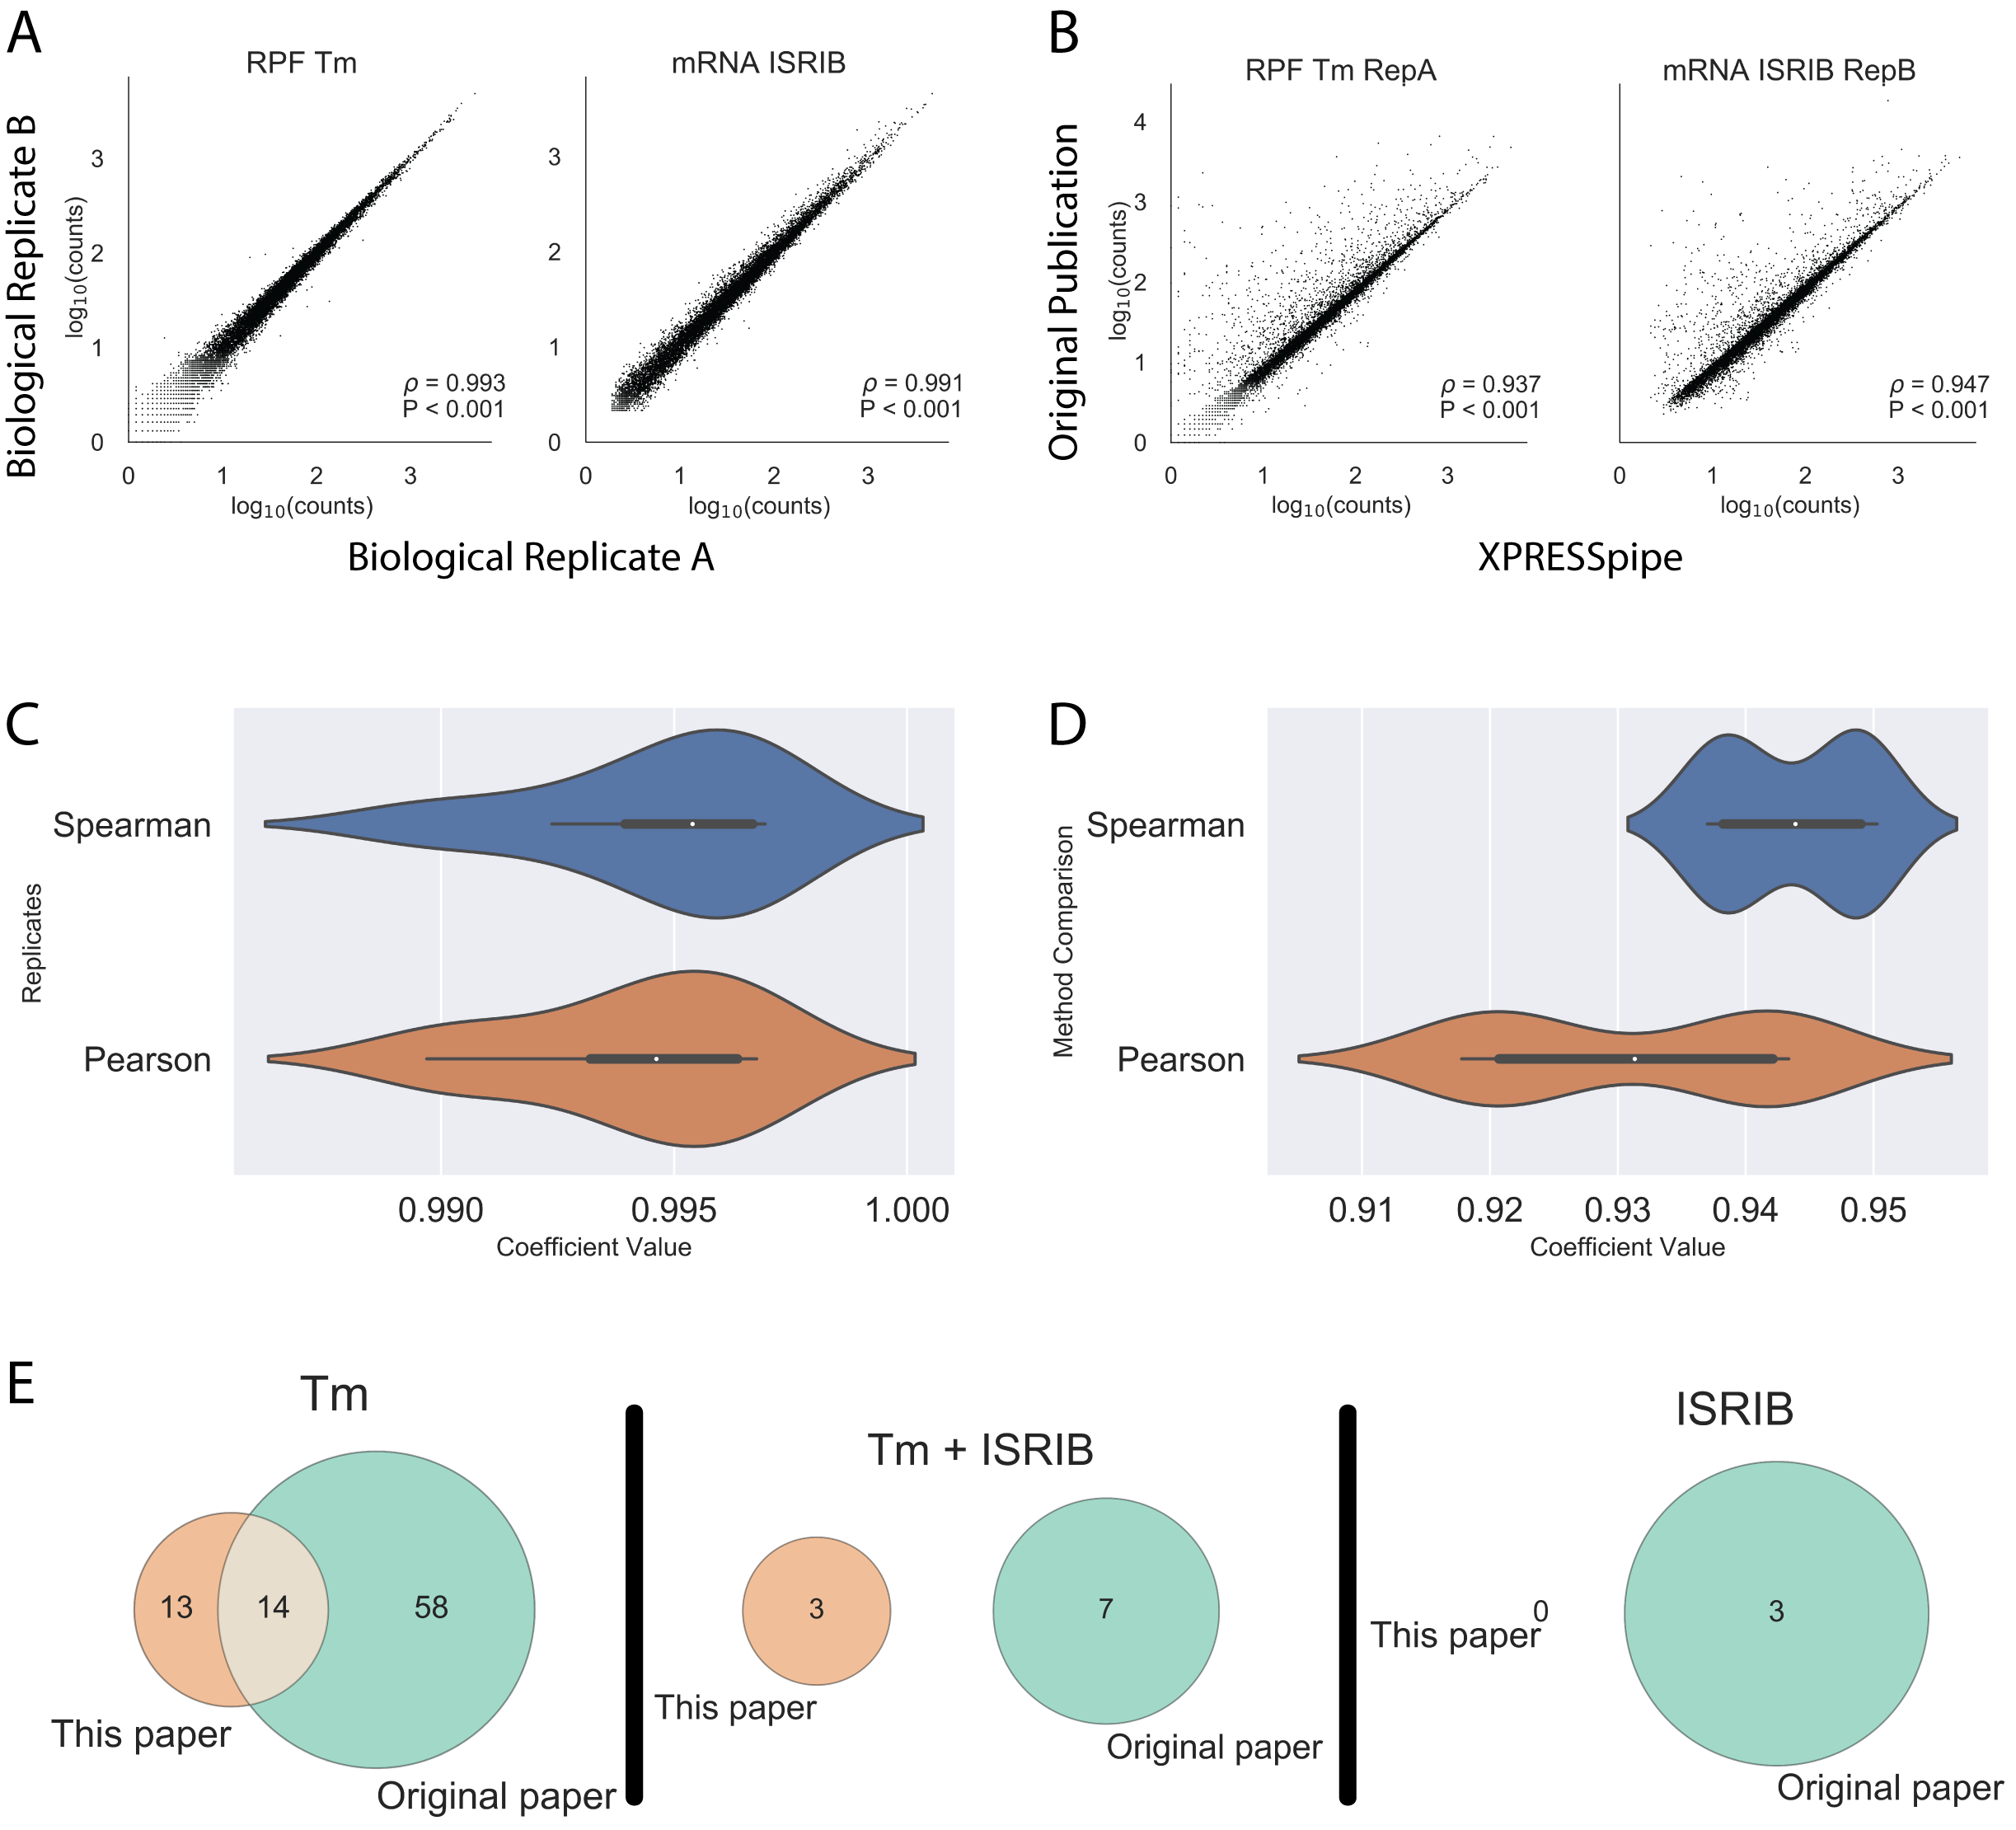
\includegraphics[width=145mm]{figures/xpresspipe_figure2.png}
  \caption{\textbf{Representative comparisons between processed data produced by XPRESSpipe and original study.} Genes were eliminated from analysis if any RNA-Seq sample for that gene had fewer than 10 counts. A) Representative comparisons of biological replicate read counts processed by XPRESSpipe. B) Representative comparisons of read counts per gene between count data from the original study and the same raw data processed and quantified by XPRESSpipe. C) Boxplot summaries of Spearman $\rho$ and Pearson r values for biological replicate comparisons. D) Boxplot summaries of Spearman $\rho$ and Pearson r values for between method processing. RPF, ribosome-protected fragments. Tm, tunicamycin. All $\rho$ values reported in A and B are Spearman correlation coefficients using RPM-normalized count data. Pearson correlation coefficients were calculated using log\textsubscript{10}(rpm(counts) + 1) transformed data. XPRESSpipe-processed read alignments were quantified to \textit{Homo sapiens} build CRCh38v96 using a protein-coding only, truncated GTF.}
  \label{fig:figure2}
\end{figure*}

\begin{figure*}
\centering
  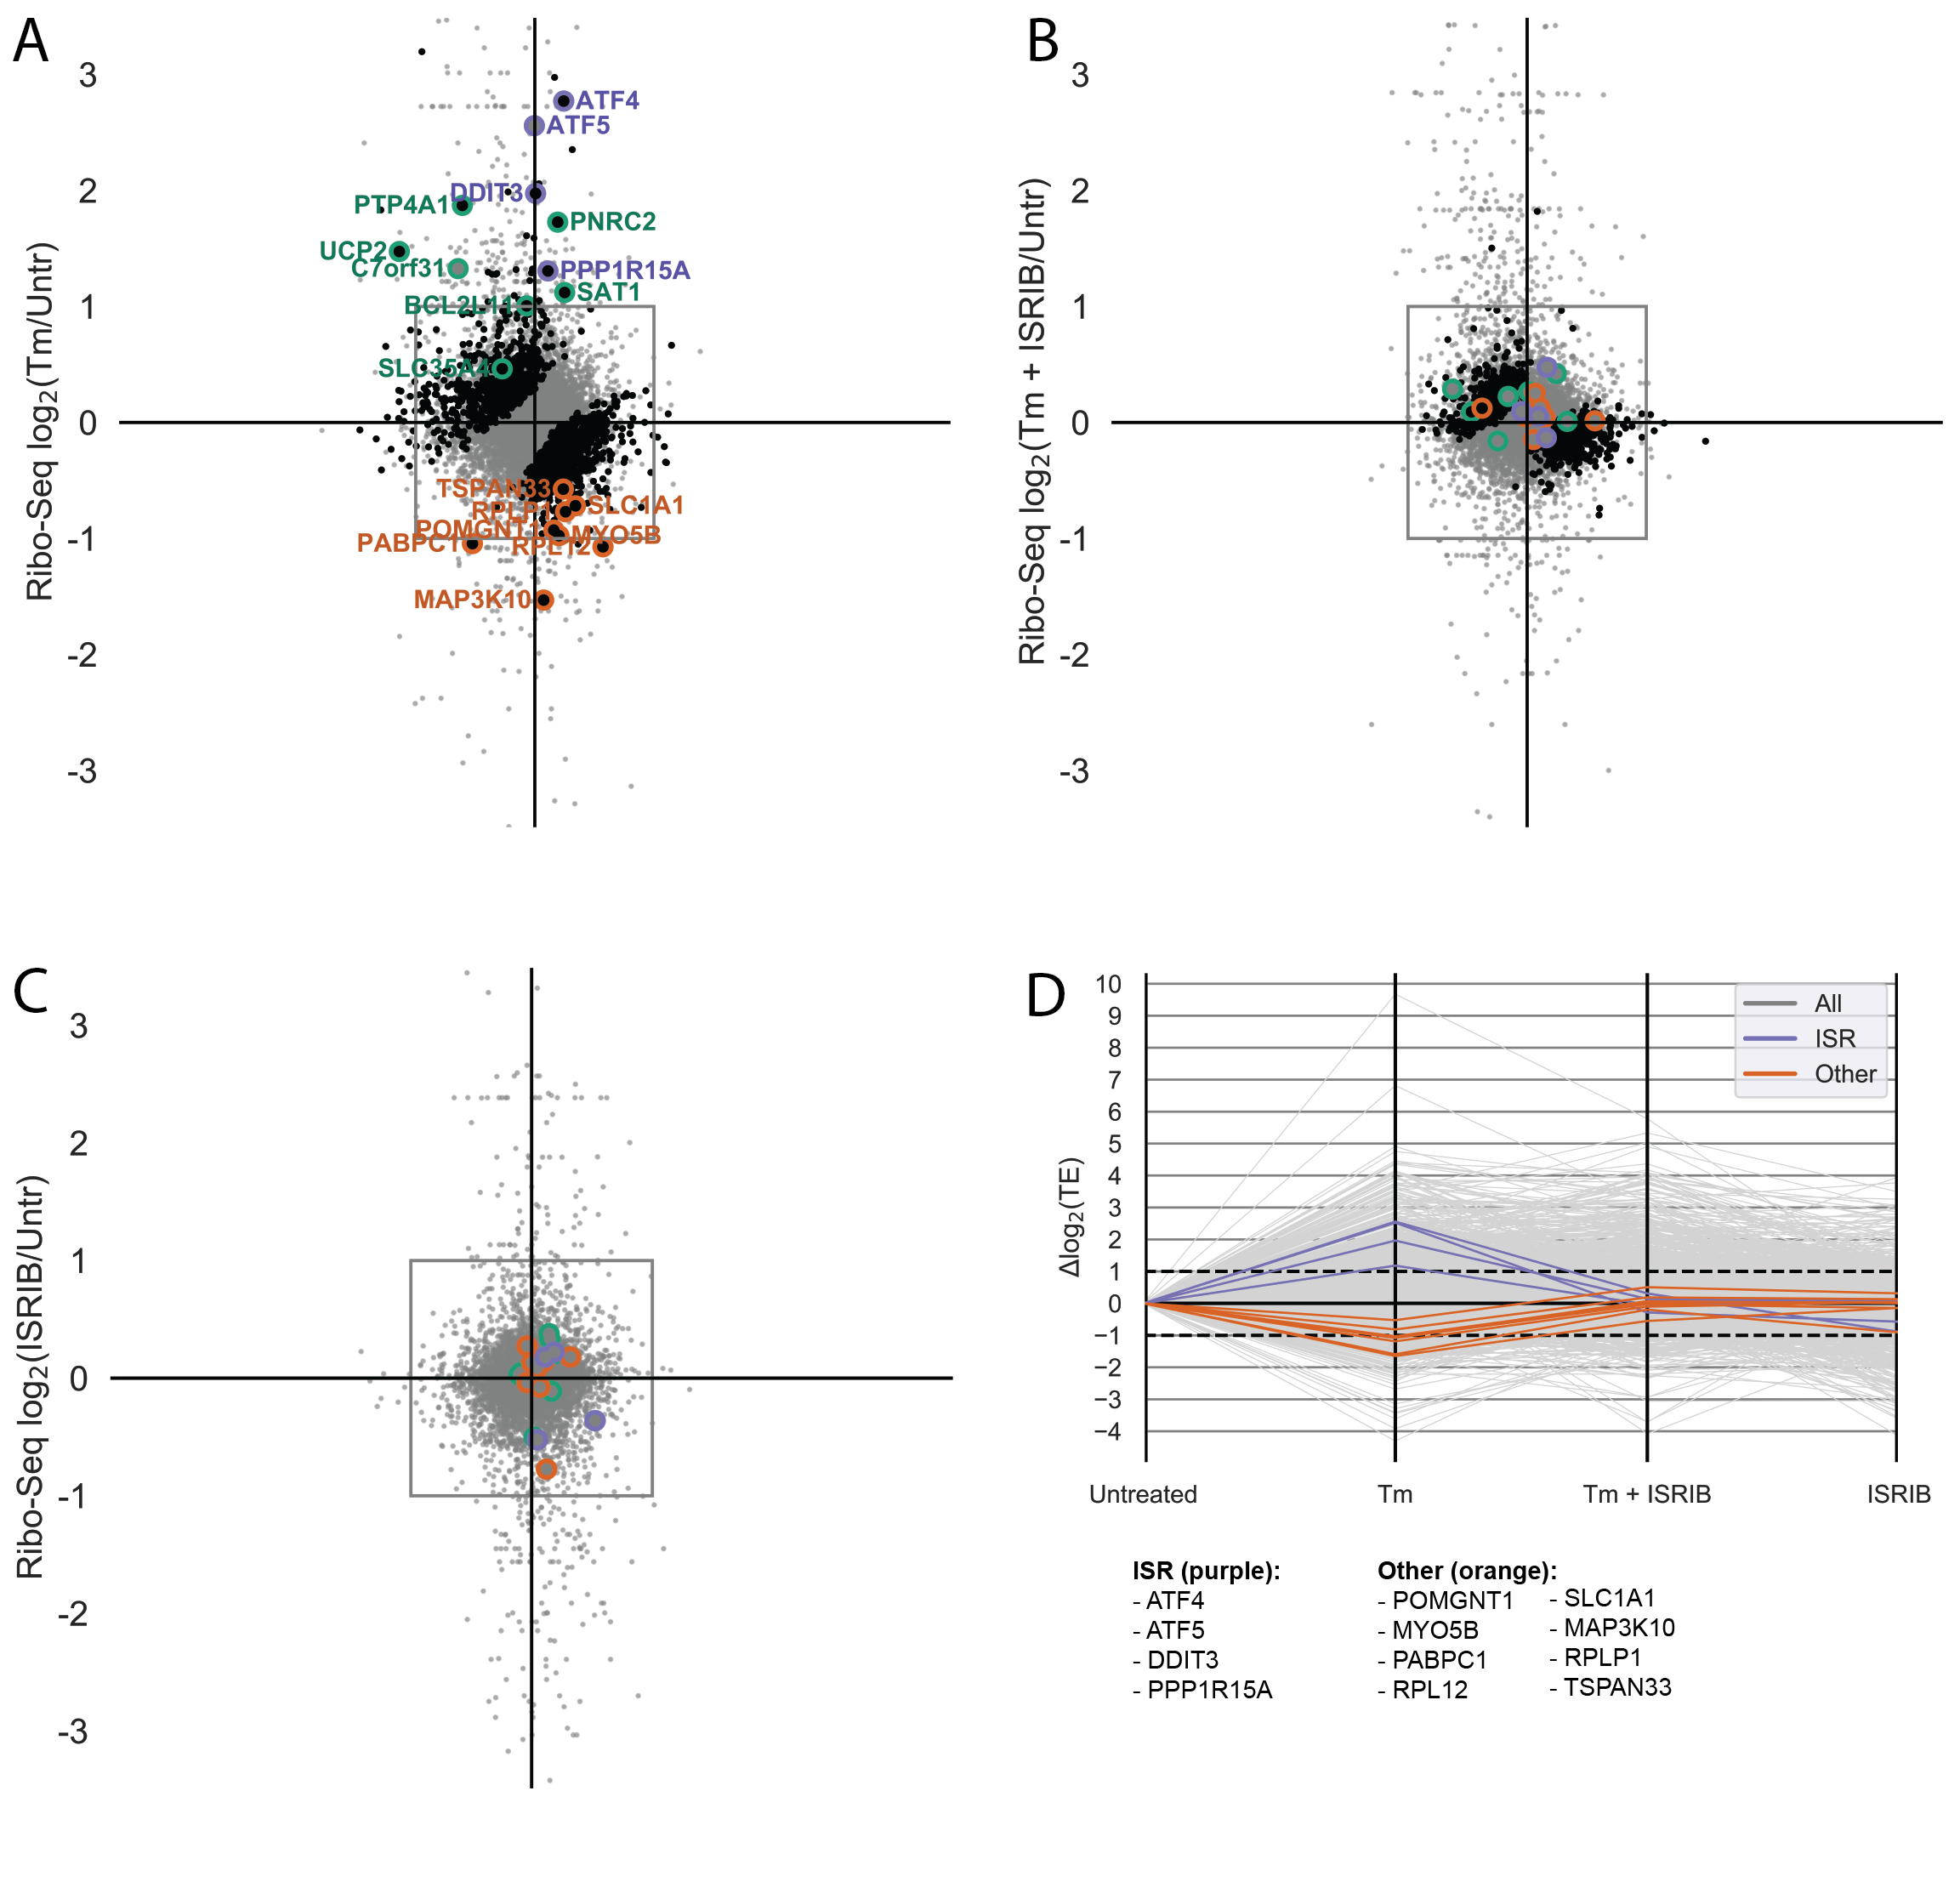
\includegraphics[width=180mm]{figures/xpresspipe_figure3.png}
  \caption{\textbf{Analysis of previously published ISR TE data using XPRESSpipe.} A-C) log\textsubscript{2}(Fold Change) for each drug condition compared to untreated for the ribosome profiling and RNA-Seq data. Purple, ISR canonical targets highlighted in the original study. Green, genes with uORFs affected by ISR as highlighted in the original study. Orange, genes fitting a strict thresholding paradigm to identify genes that display a 2-fold or greater increase in TE in Tm + ISRIB treatment compared to Tm treatment. Black, genes with statistically significant changes in TE. Grey, all genes. Changes in ribo-seq and mRNA-Seq were calculated using DESeq2. TE was calculated using DESeq2. Points falling outside of the plotted range are not included. D) Changes in log\textsubscript{2}(TE) for each drug condition compared to untreated control. Grey, all genes. Purple, ISR targets identified in the original study. Orange, genes fitting a strict thresholding paradigm to identify genes that display a 2-fold or greater increase in TE in Tm + ISRIB treatment compared to Tm treatment. XPRESSpipe-processed read alignments were quantified to \textit{Homo sapiens} build CRCh38v96 using a protein-coding only, truncated GTF.}
  \label{fig:figure3}
\end{figure*}

Similar canonical targets of translation regulation during ISR were identified in the XPRESSpipe-processed data as were identified in the original study. These targets include ATF4, ATF5, PPP1R15A, and DDIT3 (Figure \ref{fig:figure3}A-C, highlighted in purple) \cite{isrib_riboseq}. Of note, the fold-change in ribosome occupancy of ATF4 (6.83) from XPRESSpipe-processed samples closely mirrored the estimate from the original publication (6.44). Other targets highlighted in the original study \cite{isrib_riboseq}, such as ATF5, PPP1R15A, and DDIT3 also demonstrated comparable increases in their ribosome occupancy fold-changes to the original publication count data (XPRESSpipe: 5.90, 2.47, and 3.94; respectively. Original: 7.50, 2.70, and 3.89; respectively) (Figure \ref{fig:figure3}A). Similar to the originally processed data, all of these notable changes in ribosome occupancy return to untreated levels during Tm + ISRIB co-treatment (Figure \ref{fig:figure3}B). Additional ISR targets containing micro-ORFs described in the study (highlighted in green in Figure \ref{fig:figure3}A-C) were also similar in translational and transcriptional regulation across conditions between the two analyses. \par

Both the original study and our XPRESSpipe-based re-analysis show that ISRIB can counteract the significant increase in TE for a set of genes during ISR. To further explore TE regulation during ISR, we asked if ISRIB has a similar muting effect on genes with significant decreases in TE induced by the ISR. In the original study, genes with significant decreases in TE were reported in a source-data table but not a focus in the study. However, re-analysis of these data with the updated XPRESSpipe methodology identifies genes whose translational down-regulation may play a role in the neurodegenerative effects of ISR and the neuroprotective properties of ISRIB \cite{isrib_neuroprotective,isrib_neuroprotective2,isrib_neuroprotective3,isrib_neuroprotective4}. Importantly, several of these genes were not identified as having significantly down-regulated TEs in the original analysis, which suggests why a focus on translational downregulation may have been foregone. In all, we identified seven genes with the regulatory paradigm of interest: significant decreases in TE during tunicamycin-induced ISR that are rescued or overexpressed in the ISR + ISRIB condition (Table \ref{tab:targets}, descriptions sourced from \cite{genecards, ncbi, uniprot} (Figure \ref{fig:figure3}D). RNA-Seq and ribosome-footprint coverage across these genes show that the significant changes in their TE are due to neither spurious, high-abundance fragments differentially present across libraries nor variance from an especially small number of mapped reads (Figure \ref{fig:supplement6}). This is an important consideration as the commonly suggested use of the CircLigase enzyme in published ribosome profiling library preparation protocols, which circularizes template cDNA before sequencing, can bias certain molecules' incorporation into sequencing libraries based on read-end base content alone \cite{circligase_bias}. \par

Five (POMGNT1, RPL27, TKT, HSPA8, NDUFA11) out of the seven identified genes have annotated neurological functions or mutations in which lead to severe neurological disorders. Several of these disorders are directly tied to central carbon metabolism. Mutations in one other gene (RPS15A) generally present with metabolic disorders. None of these genes were identified as of interest in the original study using original methods; however, when re-processing the original count data provided with the original manuscript with DESeq2 \cite{deseq2} and the same expression pattern thresholding, four of these genes are present in the analysis (RPL27, TKT, HSPA8, RPS15A) \ref{fig:supplement7}. These observations suggest their regulation may be functionally important for the neurodegenerative effects of ISR and the neuroprotective properties of ISRIB. For example, NDUFA11 and TKT are two protein-coding genes whose functions are integrally tied to central carbon metabolism. NDUFA11 forms a subunit of mitochondrial complex I and TKT encodes a thiamine-dependent enzyme which channels excess sugars phosphates into glycolysis. Mutations in TKT present diseases associated with neurological phenotypes, and mutations in NDUFA11 present severe neurodegenerative phenotypes such as brain atrophy and encephalopathy. While at this stage speculative, it is interesting that the processing of these data for this manuscript provide a very conservative list of differentially expressed genes, and that the majority of which are associated with severe neurological phenotypes. It is therefore easy to speculate that TE regulation of these targets' abundance might be important in the neurodegeneration observed in prolonged ISR conditions. ISRIB's neuroprotective effects may, therefore, stem from a recovery of one or several of these entities' protein expression to wild-type or better levels. For example, NDUFA11 knockout models are routinely used to model mitochondrial stress, which itself activates the ISR. Therefore, some mechanism of ISRIB may be allowing for recovery of NDUFA11 translation levels, explaining the neuroprotective capabilities of ISRIB. Though speculative without further validation, these ISRIB-responsive neuronal targets act as interesting cases for further validation and study in a model more representative of neurotoxic injury and disease than the HEK-293T model used in the original study. In all, this comparison demonstrates the utility of XPRESSpipe for rapid, user-friendly analysis and re-analysis of ribosome-profiling experiments in the pursuit of biological insights and hypothesis generation.\\

\begin{table*}[!]
    \centering
\captionof{table}{\textbf{Translationally down-regulated genes during acute Tm treatment with recovered regulation during Tm + ISRIB treatment.} Gene names succeeded by an asterisk indicate these genes were identified in the original data when re-analyzed with DESeq2 \cite{deseq2}. Gene names succeeded by an ampersand indicate genes with strong neurological phenotypes.}
\begin{tabular}{p{2cm}p{15cm}}
 \textbf{Gene Name} & \textbf{Relevant Description} \\
 \hline
 POMGNT1\textsuperscript{\&} & Participates in O-mannosyl glycosylation. Mutations have been associated with muscle-eye-brain diseases and congenital muscular dystrophies. Expressed especially in astrocytes, as well as in immature and mature neurons. Expressed across brain. \\
 \hline
 RPL27*\textsuperscript{\&} & Subunit of ribosome catalyzing protein synthesis. Expressed in cerebral cortex in embryonic tissue and/or stem cells. Mutations associated with Diamond-Blackfan Anemia 16, a metabolic disease, which may present with microcephaly. \\
 \hline
 TKT*\textsuperscript{\&} & Encodes thiamine-dependent enzyme that channels excess sugars phosphates to glycolysis. Mutations associated with developmental delays and Wernicke-Korsakoff Syndrome, a metabolic and neuronal disease and associated with encephalopathy and dementia-like characteristics. \\
 \hline
 HSPA8*\textsuperscript{\&} & Encodes heat shock protein 70 member. Facilitates protein folding and localization. Diseases associated with mutations include Auditory System Disease and Brain Ischemia, both neurological disorders. Expressed in cerebral cortex in embryonic tissue and/or stem cells. \\
 \hline
 NDUFA11\textsuperscript{\&} & Encodes subunit of mitochondrial complex I, a vital part of the electron transport chain. Mutations associated with severe mitochondrial complex I deficiency. Related pathways include the GABAergic synapse. Associated diseases include brain atrophy, encephalopathy, and leber hereditary optic neuropathy. Overexpressed in frontal cortex. \\
 \hline
 HIST2H3D & Responsible for the nucleosome structure. No neurological descriptions currently known. \\
 \hline
 RPS15A* & Subunit of ribosome catalyzing protein synthesis. Diseases associated include Diamond-Blackfan Anemia, an inborn error of metabolism disease. \\
 \label{tab:targets}
\end{tabular}
\end{table*}

\subsection*{Cost Analysis and Performance}
XPRESSpipe functions can be computationally intensive, and thus, super-computing resources are recommended, especially when handling large datasets or when aligning to larger, more complex genomes. Many universities provide super-computing resources to their affiliates; however, in cases where these resources are not available, servers such as Amazon Web Services (AWS) \cite{aws} can be used to process sequencing data using XPRESSpipe. Table \ref{tab:chpc_performance} outlines runtime statistics for the ISRIB dataset used in this study. The ISRIB ribosome profiling dataset contained a total of 32 raw sequence files that were aligned to \textit{Homo sapiens}, thus it acts as a high-end estimate of the time required to process data with XPRESSpipe. For a comparable dataset, cost to use an AWS computational node with similar specifications for the above elapsed time would be approximately 13.33 USD using an Amazon EC2 On-Demand m5.4xlarge node (however, significantly reduced rates are available if using Spot instances or by using the free tier) and storage cost would amount to around 11.5 USD/month on Amazon S3 storage (although much of the intermediate data does not need to be stored long term; however, input raw data should always be archived). \\

\begin{table*}[h]
    \centering
\captionof{table}{\textbf{XPRESSpipe sub-module statistics for dataset GSE65778.} \texttt{geneCoverage} module performed on high-coverage gene.}
\begin{tabular}{p{5cm}p{3.5cm}p{2.7cm}p{1.8cm}}
\textbf{Process} & \textbf{Command} & \textbf{Wallclock Time} & \textbf{Max RAM}\\
  \hline
  Curate STAR reference & \texttt{curateReference} & 00h 37m 10.15s & 34.03gb \\
  \hline
  Truncate GTF & \texttt{modifyGTF -t} & 00h 03m 15.86s & 03.25gb \\
  \hline
  Read Pre-processing & \texttt{trim} & 00h 20m 10.78s & 00.45gb \\
  \hline
  Alignment and Post-processing & \texttt{align} &  & \\
  \hline
  Quantification & \texttt{count -c htseq} &  & \\
  \hline
  Isoform Abundance & \texttt{count -c cufflinks} &  & \\
  \hline
  Differential Expression (n=9) & \texttt{diffxpress} &  & \\
  \hline
  Read Distributions & \texttt{readDistribution} &  & \\
  \hline
  Metagene Analysis & \texttt{metagene} &  & \\
  \hline
  Gene Coverage (n=1) & \texttt{geneCoverage} &  & \\
  \hline
  Periodicity & \texttt{periodicity} &  & \\
  \hline
  Library Complexity & \texttt{complexity} &  & \\
  \hline
  rRNA probe & \texttt{rrnaProbe} &  & \\
  \hline
  Pipeline & \texttt{riboseq} & & \\
  \hline
  & & & \\
  \hline
  \hline
  \textbf{Attribute} & & & \textbf{Value}\\
  \hline
  Total Raw Input & & & 257 GB \\
  \hline
  Total Output & & & 500 GB \\
  \hline
  Allocated CPUs & & & 16 \\
  \hline
  Allocated Memory & & & 64GB \\
 \label{tab:chpc_performance}
\end{tabular}
\end{table*}

\section*{Availability and Future Directions}
We have described a new software suite, XPRESSyourself, a reference implementation of correct ribosome profiling data analysis built upon of a synthesis of new tools, old tools, and automated pipelines to aid in the processing and analysis of these data. XPRESSyouself is perpetually open source and protected under the GPL-3.0 license. Updates to the software are version controlled and maintained on GitHub \cite{xpressyourself}. Jupyter notebooks and video walkthroughs are included within the README files at \cite{xpressyourself}. Documentation is hosted on readthedocs \cite{readthedocs} at \cite{xpresspipe_docs} and \cite{xpressplot_docs}. Source code for associated analyses and figures for this manuscript can be accessed at \cite{manuscript}. The data used in this manuscript are available under the Gene Expression Omnibus persistent identifier GSE65778 \cite{isrib_geo} for ribosome profiling data and under the dbGaP Study Accession persistent identifier phs000178 \cite{tcga_data} for the TCGA data.\par

Although RNA-Seq technologies are quite advanced, standardized computational protocols are much less established for ribosome profiling. As we discussed in this manuscript, this becomes problematic when individuals or groups are not using the most up-to-date or complete methods or may not be aware of particular biases or measures of quality control required to produce a reliable, high-quality sequencing study. XPRESSpipe handles these issues through on-going curation of benchmarked software tools and by simplifying the required user input. It also outputs all necessary quality control metrics so that the user can quickly assess the quality of their data and identify any systematic problems or technical biases that may compromise their analysis. Video walkthroughs, example scripts, and interactive command builders are available within this software suite to make these analyses accessible to exprienced and inexperienced users alike. XPRESSyourself will enable individuals and labs to process and analyze their own data, which will result in quicker turnaround times of experiments and financial savings.\par

One particular benefit of XPRESSyourself is that it consolidates, streamlines, and/or introduces many tools specific to ribosome profiling processing and analysis. This includes curating GTF files with $5'$- and $3'$- truncated CDS annotations, rRNA probe design for subtractive hybridization of abundant rRNA contaminants, automated quality-control analyses to report on ribosome footprint periodicity and metagene coverage, and intron-less gene coverage profiles. These tools will help to democratize aspects of ribosome profiling for which software have not been previously publicly available.\par

We demonstrated the utility of the XPRESSyourself toolkit by re-analyzing a publicly available ribosome profiling dataset. From this analysis, we identified putative translational regulatory targets of the integrated stress response (ISR) that may contribute to its neurodegenerative effects and their rescue by the small-molecule ISR inhibitor, ISRIB. This highlights the importance of re-analyzing published datasets with more current methods, as improved analysis methodologies and updated organism genome references may result in new interpretations and hypotheses. \par

With the adoption of this flexible pipeline, the field of high-throughput sequencing, particularly ribosome profiling, can continue to standardize the processing protocol for associated sequence data and eliminate the variability that comes from the availability of a variety of software packages for various steps during sequence read processing. Additionally, XPRESSpipe consolidates various tools used by the ribosome profiling and RNA-Seq communities. With these tools, genome reference formatting and curation is automated and accessible to the public. Adoption of this tool will allow scientists to quickly process and access their data independently, guide them in understanding key considerations in processing their data, and standardize protocols for ribosome profiling and other RNA-Seq applications, thus increasing the reproducibility of sequencing analyses. \\

\begin{table}[!]
    \centering
\captionof{table}{\textbf{Software Description}}
\begin{tabular}{p{4cm}p{9cm}}
 Project Name & XPRESSyourself \\
 \hline
 Project Home Page & https://github.com/XPRESSyourself \\
 \hline
 Archived Versions DOIs & 10.5281/zenodo.3338669, 10.5281/zenodo.3337897 \\
 \hline
 Operating Systems & macOS, Linux, centOS \\
 \hline
 Programming Languages & Python, R \\
 \hline
 Other Requirements & Anaconda \\
 \hline
 License & GNU General Public License v3.0 \\
\end{tabular}
\end{table}

\section*{List of Abbreviations}
AWS - Amazon Web Services,
BAM - Binary Sequence Alignment Map,
BED - Browser Extensible Data,
cDNA - complementary DNA,
CDS - coding sequence of gene,
ChIP-seq - chromatin immunoprecipitation sequencing,
CPU - central processing unit,
dbGaP - Database of Genotypes and Phenotypes,
DNA - deoxyribonucleic acid,
FDR - false discovery rate,
FPKM - fragments per kilobase of transcript per million,
GEO - Gene Expression Omnibus,
GTF - General Transfer Format,
IGV - Integrative Genomics Viewer,
ISR - integrated stress response,
ISRIB - ISR inhibitor,
mRNA - messenger RNA,
nt - nucleotide,
PCA - principal component analysis,
PCR - polymerase chain reaction,
RAM - random access memory,
RNA - ribonucleic acid,
RNA-Seq - RNA sequencing
RPKM - reads per kilobase of transcript per million,
RPM - reads per million,
rRNA - ribosomal RNA,
TCGA - The Cancer Genome Atlas,
TE - translation efficiency,
TPM - transcripts per million,
UMI - unique molecular identifier,
UTR - untranslated region\\

\section*{Ethics Approval and Consent to Participate}
Protected TCGA data were obtained through dbGaP project number 21674 and utilized according to the associated policies and guidelines.\\

\section*{Consent for Publication}
Protected TCGA data were obtained through dbGaP project number 21674 and utilized according to the associated policies and guidelines.\\

\section*{Competing Interests}
The authors declare that they have no competing interests.\\

\section*{Funding}
J.A.B. received support from the National Institute of Diabetes and Digestive and Kidney Diseases (NIDDK) Inter-disciplinary Training Grant T32 Program in Computational Approaches to Diabetes and Metabolism Research, 1T32DK11096601 to Wendy W. Chapman and Simon J. Fisher. J.T.M. received support as an HHMI Fellow of the Jane Coffin Childs Memorial Fund for Medical Research. A.J.B received support from the National Cancer Institute (NCI) Predoctoral to Postdoctoral Fellow Transition Award, K00CA212445. This work was supported by NIDDK fellowship 1T32DK11096601 (to J.A.B.) and NIH grant R35GM13185 (to J.R.). The computational resources used were partially funded by the NIH Shared Instrumentation Grant 1S10OD021644-01A1.\\

\section*{Contributions}
J.A.B. conceptualized and administered the project; performed all investigation, analysis, visualization, and data curation; provisioned resources; and wrote the original draft of this manuscript. J.A.B., J.R.B., J.T.M., and J.G. and developed the methodology. J.A.B. and J.R.B. designed and wrote the software. J.A.B., J.T.M., A.J.B., and Y.O. performed software validation. J.A.B. and J.R. acquired funding. J.R., A.R.Q., and J.G. supervised the study. All authors reviewed and edited this manuscript.\\

\begin{table*}[!]
    \centering
\captionof{table}{\textbf{Author ORCIDs}}
\begin{tabular}{p{1.5cm}p{4cm}}
 \textbf{Author} & \textbf{ORCID}\\
 \hline
 J.A.B. & 0000-0002-5096-0558 \\
 \hline
 J.R.B. & 0000-0001-5470-8299 \\
 \hline
 J.T.M. & 0000-0002-3017-8665 \\
 \hline
 Y.O. & 0000-0001-9523-1044 \\
 \hline
 A.J.B. & 0000-0003-2273-8922 \\
 \hline
 A.R.Q. & 0000-0003-1756-0859 \\
 \hline
 J.G. & 0000-0001-7568-6789 \\
 \hline
 J.R. & 0000-0002-2710-9765 \\
\end{tabular}
\end{table*}

\section*{Acknowledgments}
The authors wish to thank Michael T. Howard for helpful discussions concerning ribosome profiling and sequencing analysis. The authors also wish to thank Mark E. Wadsworth, Ryan Miller, and Michael J. Cormier for helpful discussions on pipeline design. They also wish to thank T. Cameron Waller for helpful discussions related to pipeline design and biological analysis. The support and resources from the Center for High-Performance Computing at the University of Utah are gratefully acknowledged. The results published here are in whole or part based upon data generated by the TCGA Research Network \cite{tcga}.\\

\bibliography{manubib}
\bibliographystyle{Science}

\newpage
\beginsupplement

\begin{figure}
\centering
  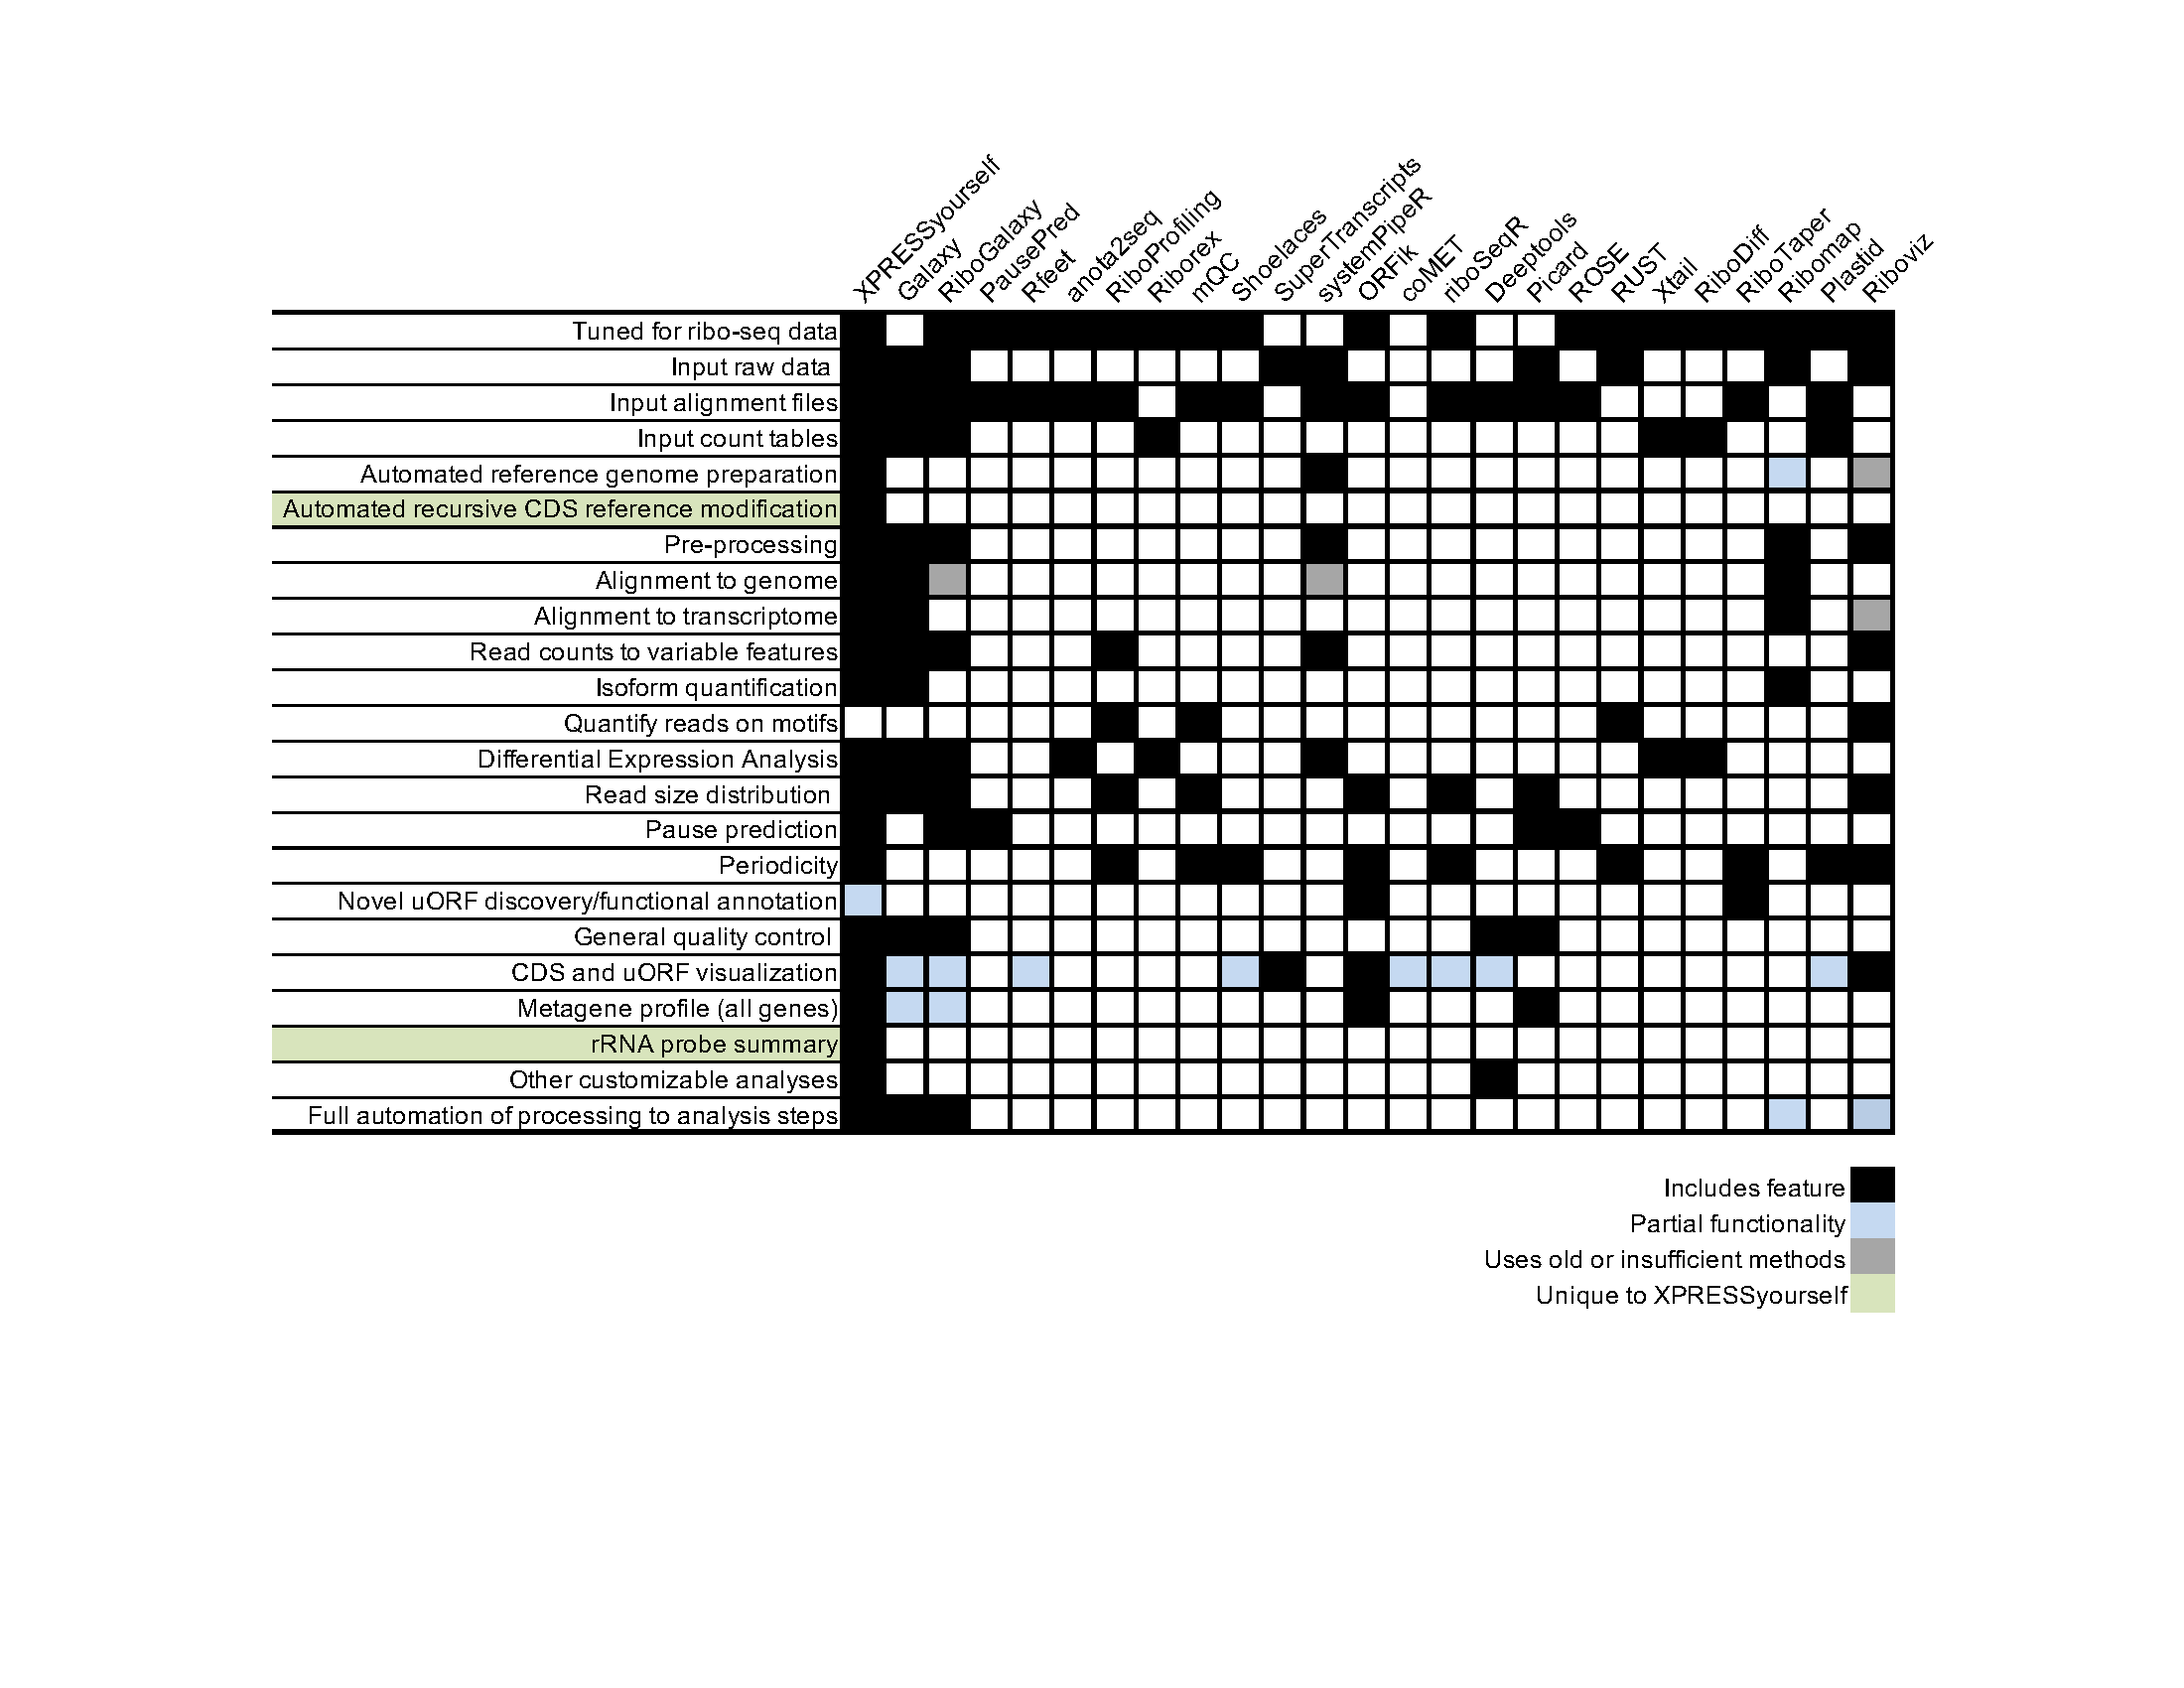
\includegraphics[width=180mm]{figures/xpresspipe_supplement1.png}
  \caption{\textbf{Comparison between XPRESSyourself and other available software packages for ribosome profiling data analysis.} Black boxes indicate full functionality, blue boxes indicate partial functionality, grey boxes indicate incomplete or outdated functionality, and white boxes indicate no functionality for the specified task. Rankings were compiled using the tools' documentation and manuscript. If a function was not clearly described in either, a white box was given.}
  \label{fig:supplement1}
\end{figure}

\begin{figure}
\centering
  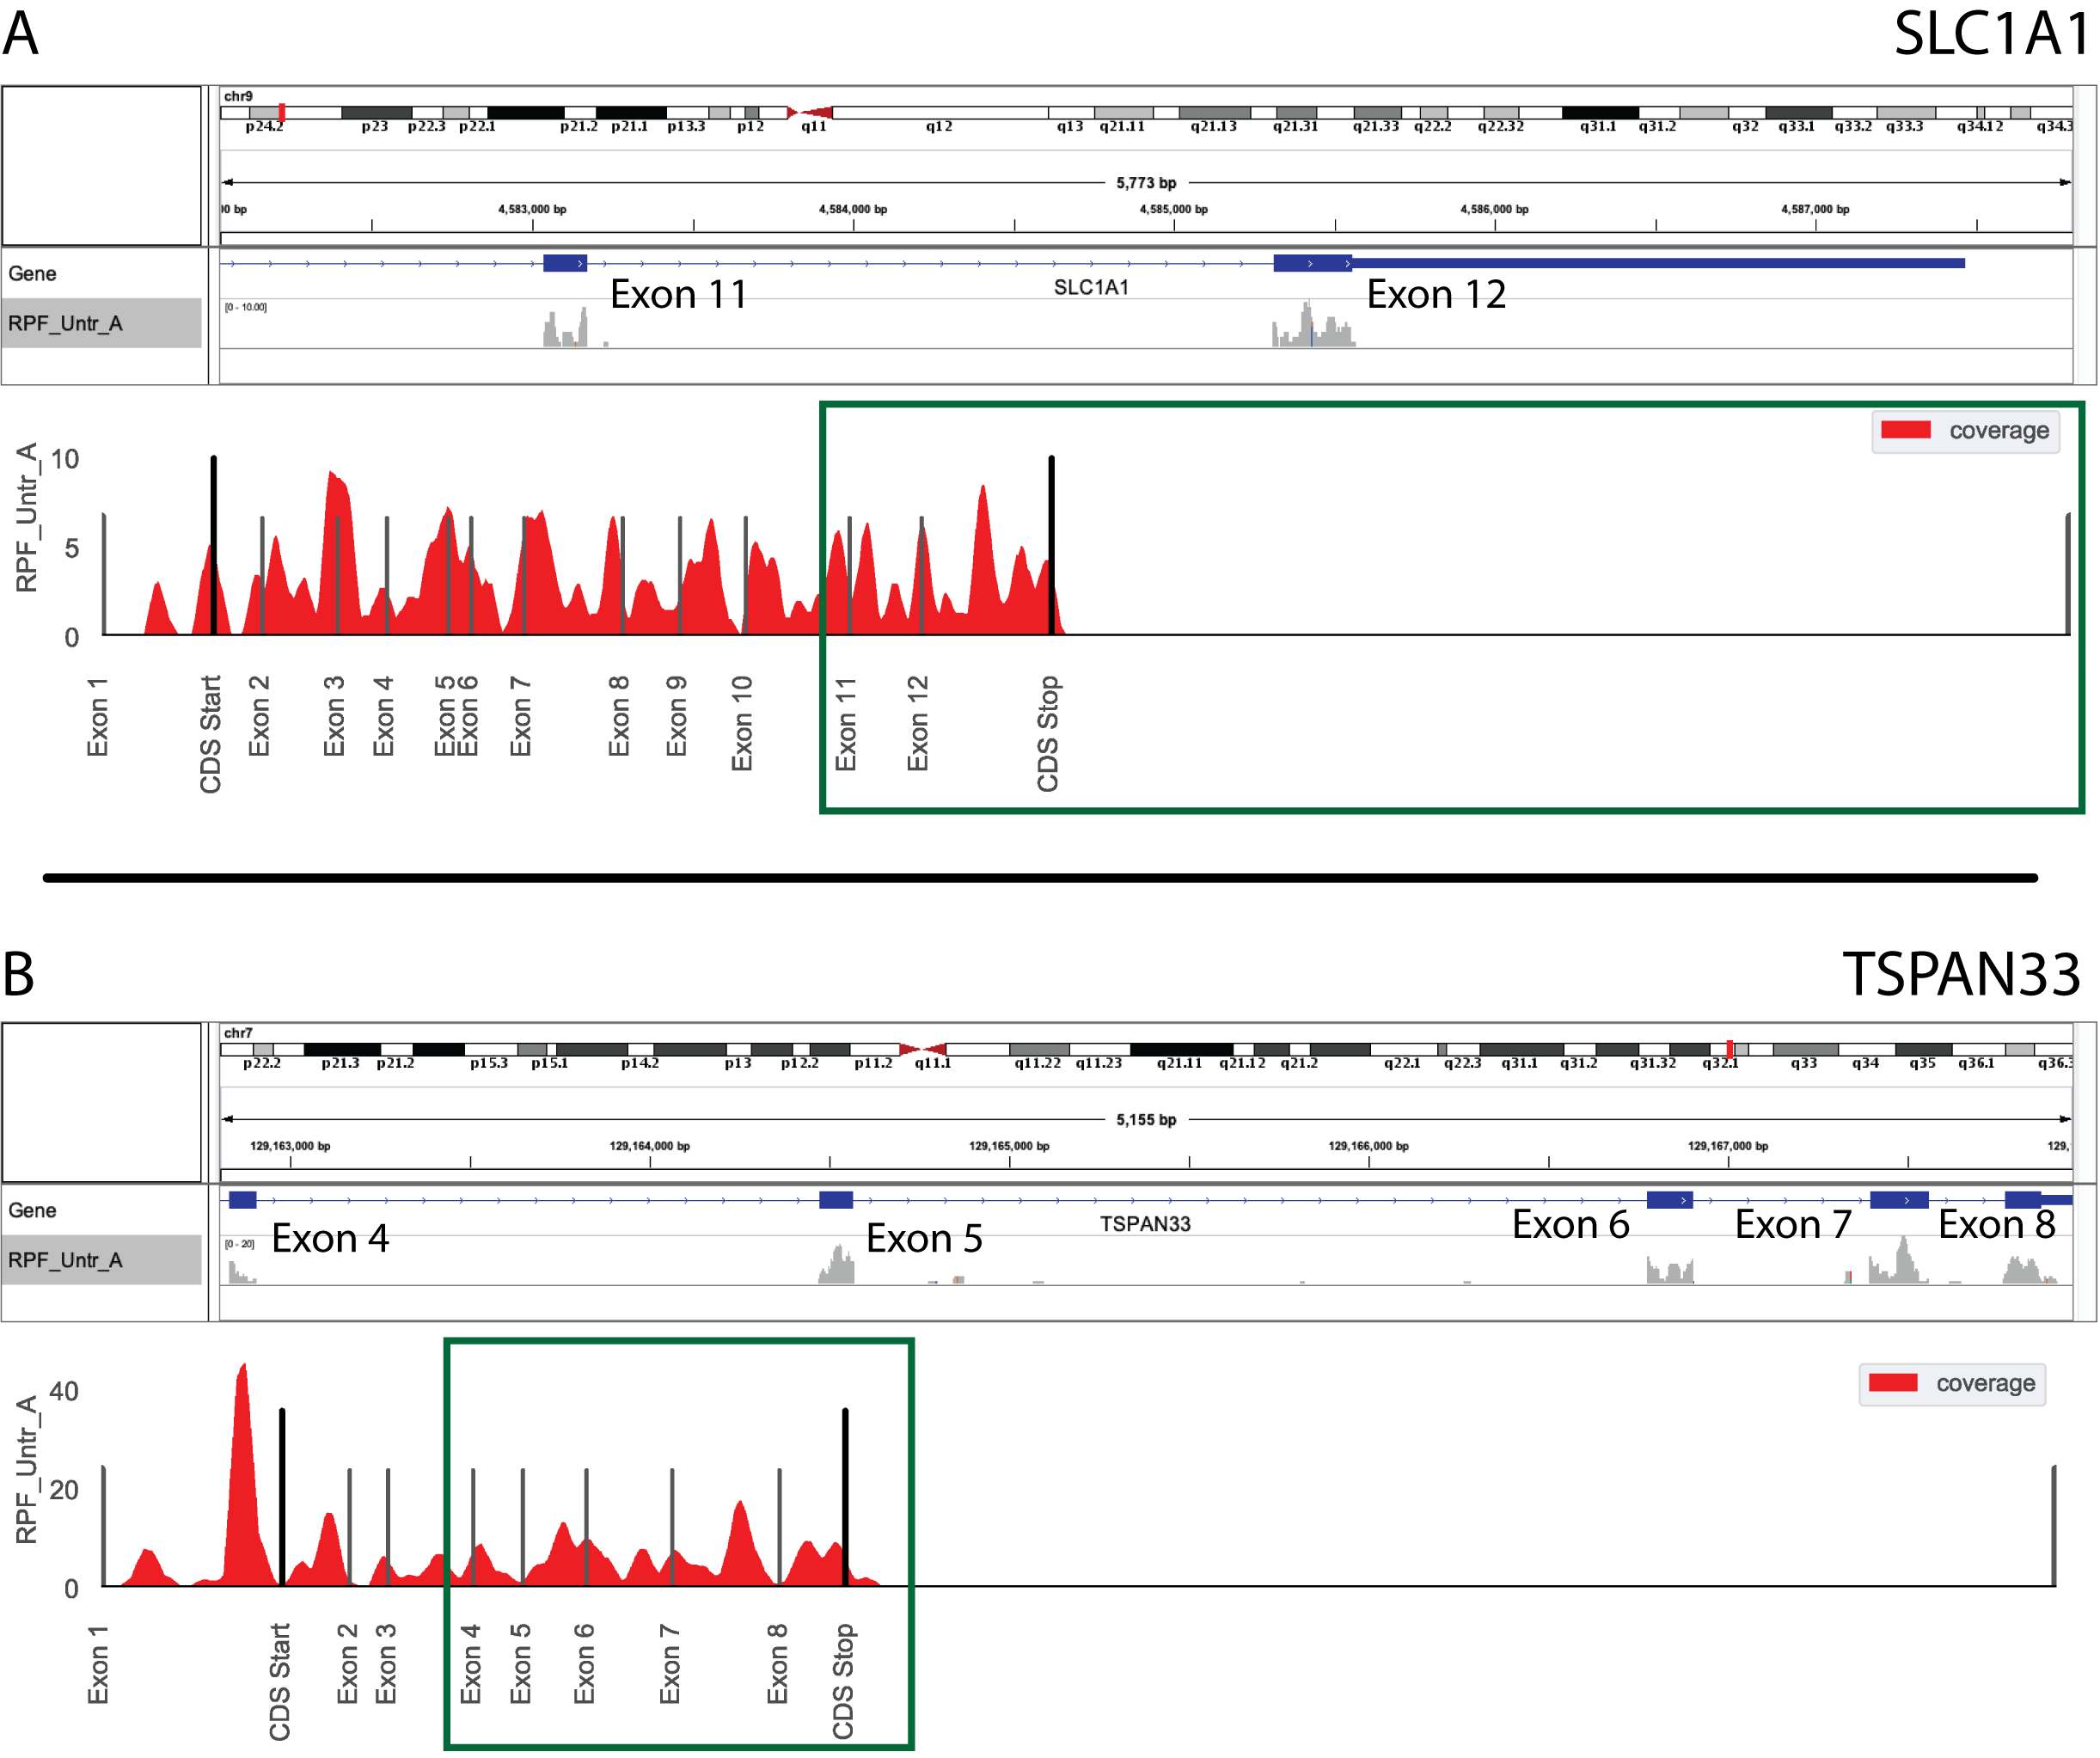
\includegraphics[width=160mm]{figures/xpresspipe_supplement2.png}
  \caption{\textbf{Comparison between IGV browser and geneCoverage output.} A) Gene coverage from IGV (above) and XPRESSpipe (below) for SLC1A1. B) Gene coverage from IGV (above) and XPRESSpipe (below) for TSPAN33. Introns collapsed by XPRESSpipe. Green box, region shown in corresponding IGV window comparing outputs between the two programs.}
  \label{fig:supplement2}
\end{figure}

\begin{figure}
\centering
  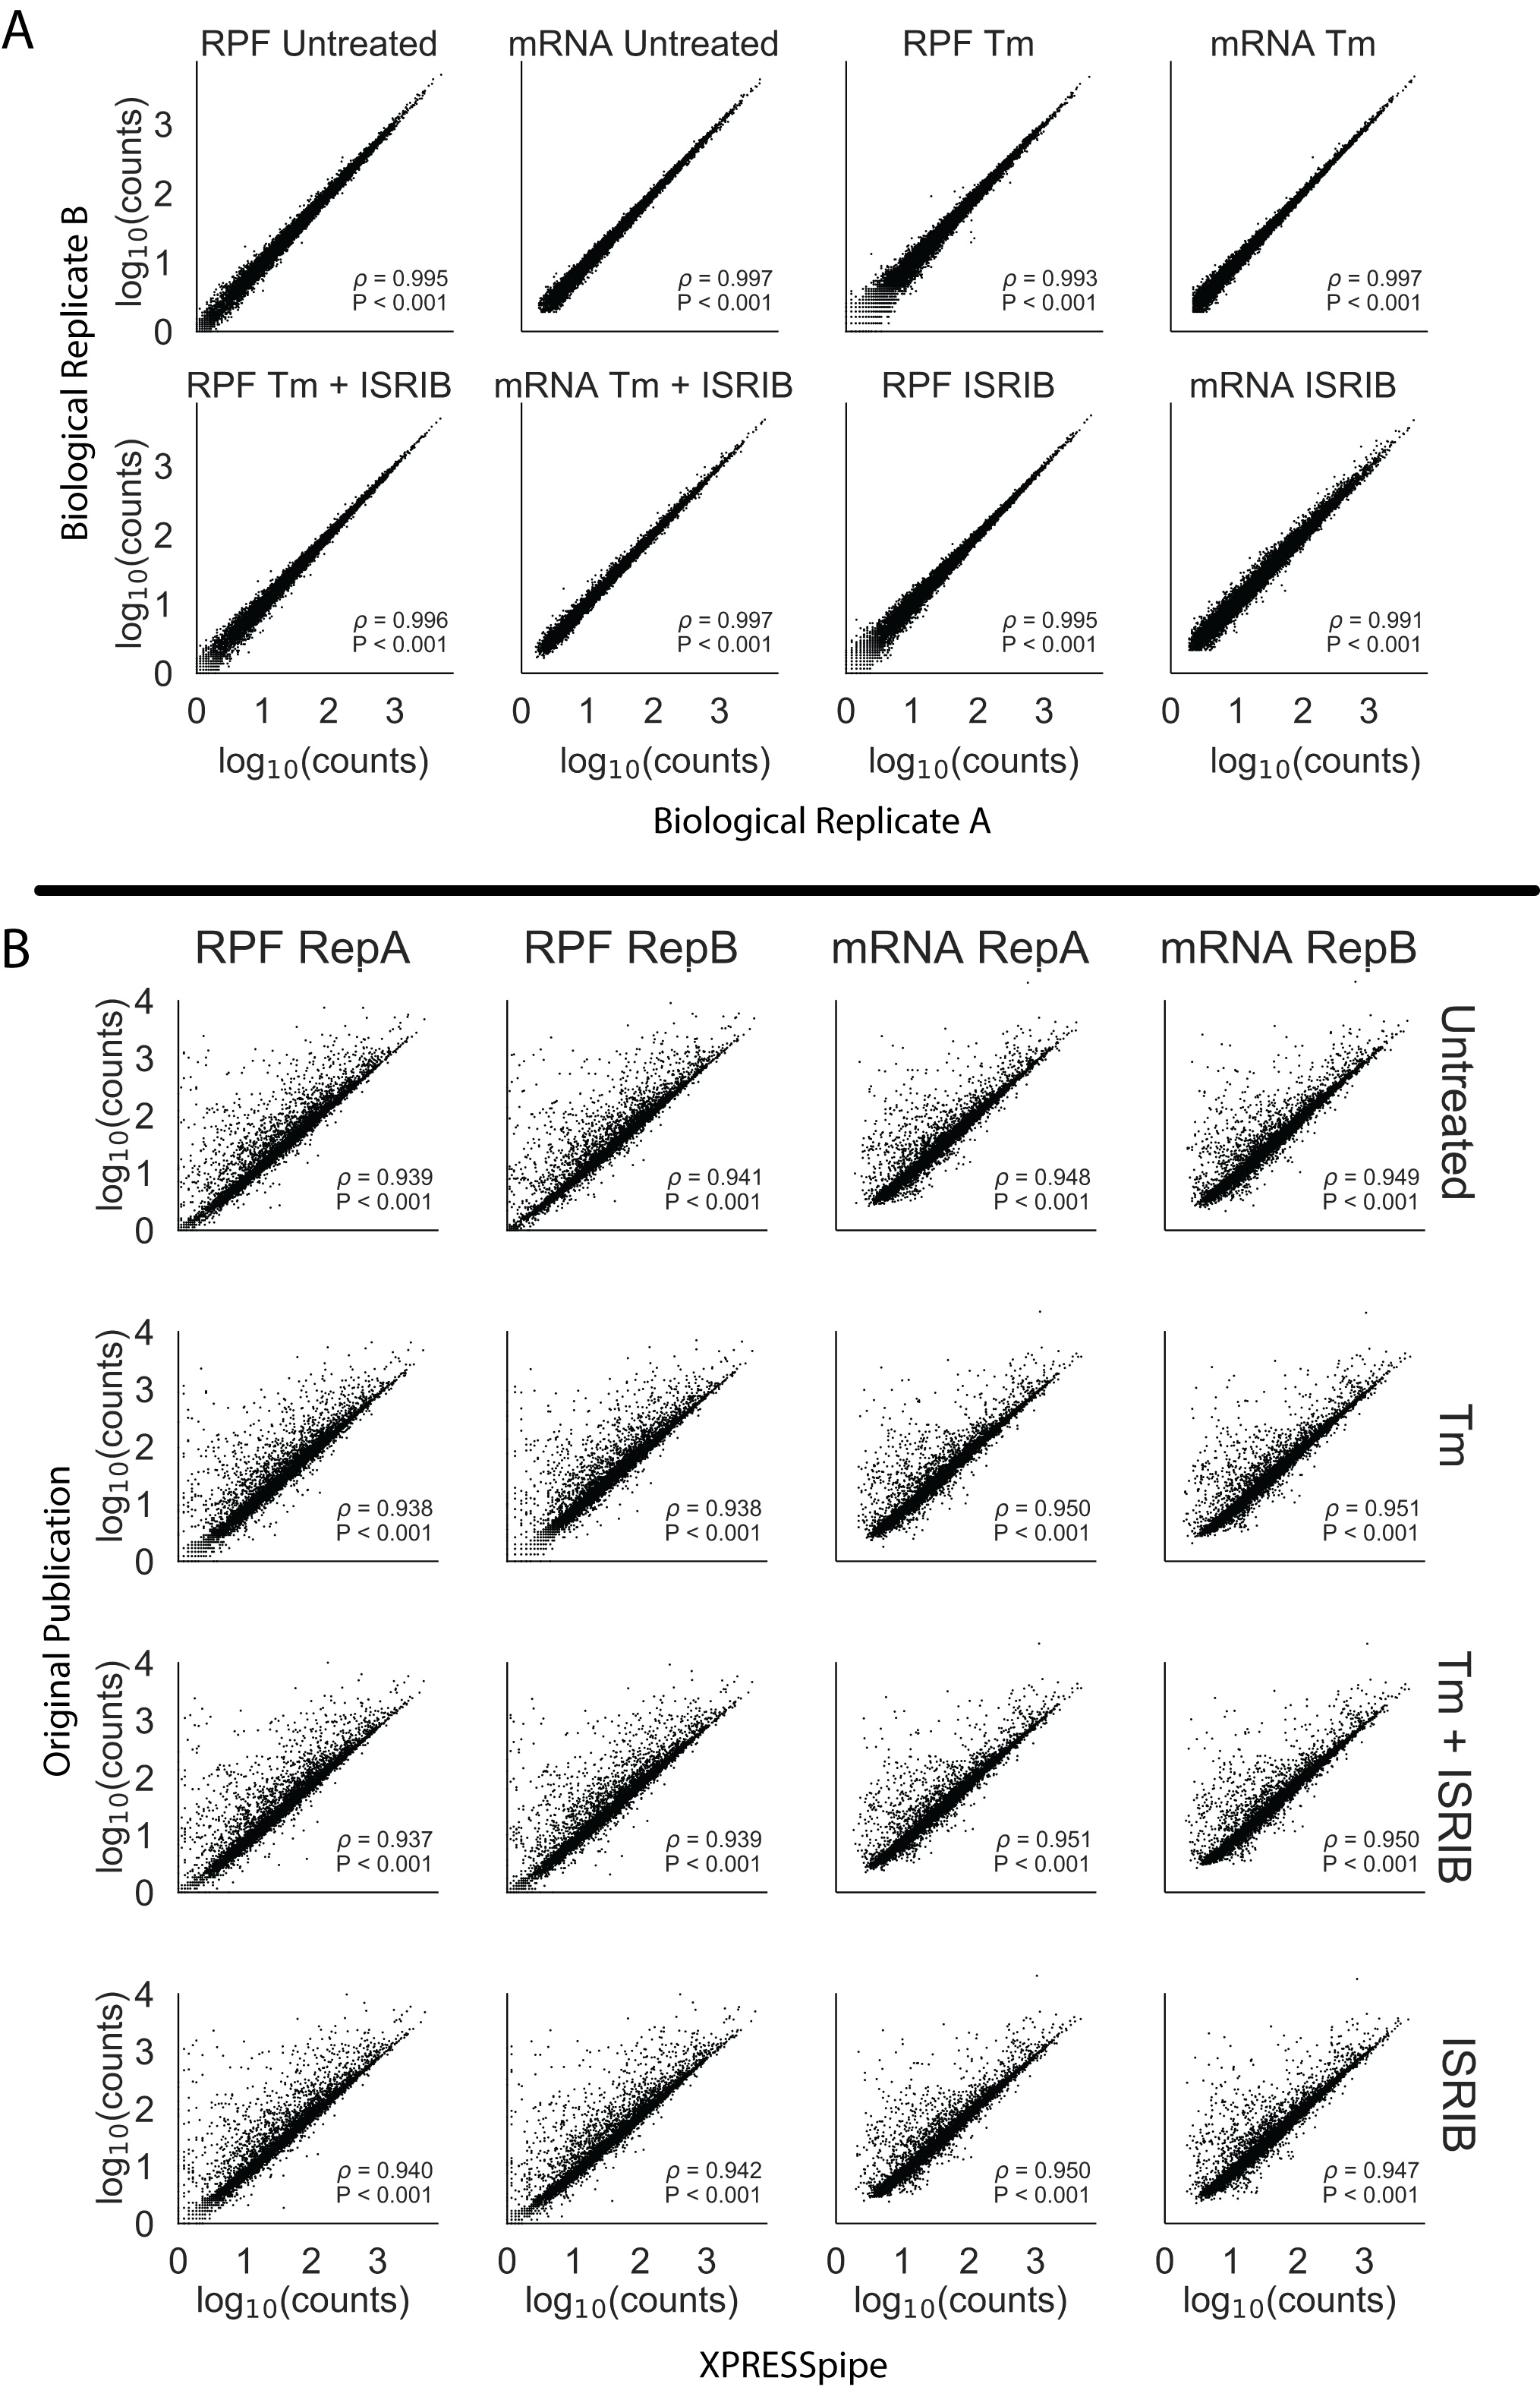
\includegraphics[width=160mm]{figures/xpresspipe_supplement3.png}
  \caption{\textbf{Comparison between processed data produced by XPRESSpipe and original study.} Genes were eliminated from analysis if any RNA-Seq sample for that gene had fewer than 10 counts. A) Comparison of biological replicate read counts processed by XPRESSpipe. B) Comparison of read counts per gene between count data from the original study and the same raw data processed and quantified by XPRESSpipe. RPF, ribosome-protected fragments. Tm, tunicamycin. All $\rho$ values reported are Spearman correlation coefficients. XPRESSpipe-processed read alignments were quantified to \textit{Homo sapiens} build CRCh38v96 using a protein-coding only, truncated GTF.}
  \label{fig:supplement3}
\end{figure}

\begin{figure}
\centering
  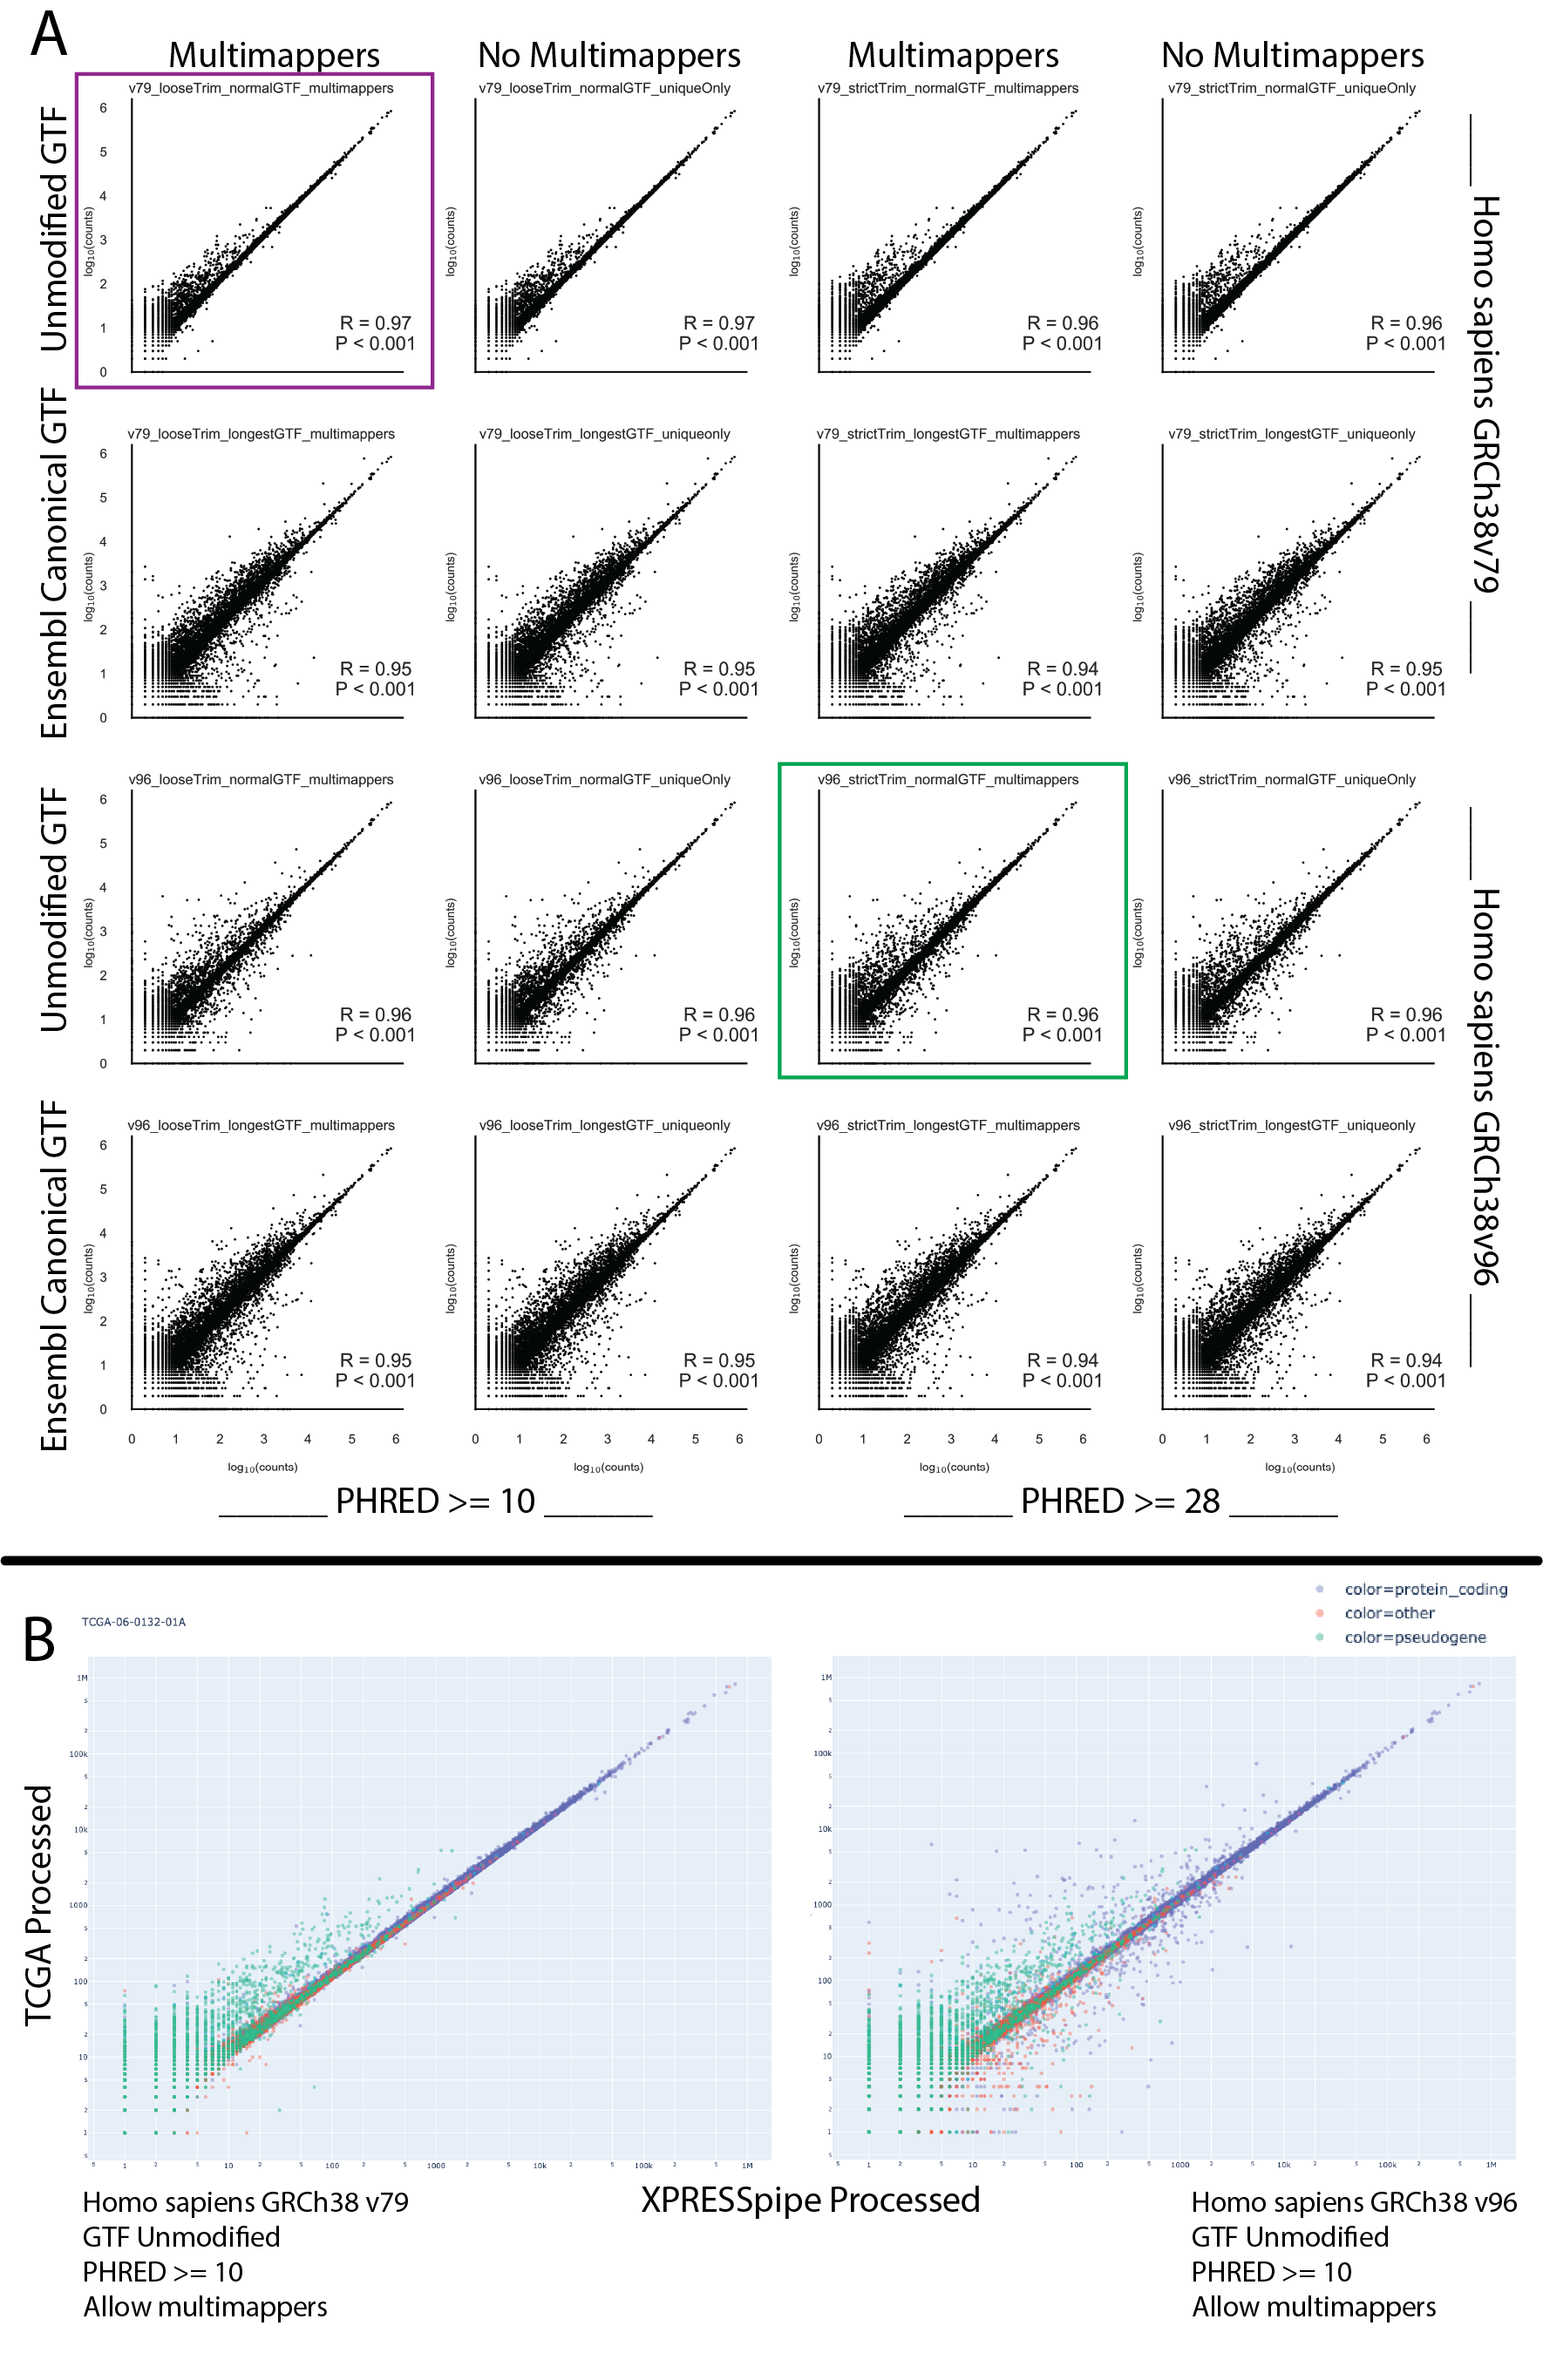
\includegraphics[width=160mm]{figures/xpresspipe_supplement4.png}
  \caption{\textbf{Original ISRIB count data plotted against XPRESSpipe-processed data reveals systematic differences between the analytical regimes.} A) Selected highlighted genes show consistent differences between processing methods. B) Spearman correlation plots using the data table provided as supplementary data with the original ISRIB manuscript comparing biological replicates. RPF, ribosome-protected footprint. Tm, tunicamycin. All $\rho$ values reported are Spearman correlation coefficients.}
  \label{fig:supplement4}
\end{figure}

\begin{figure}
\centering
  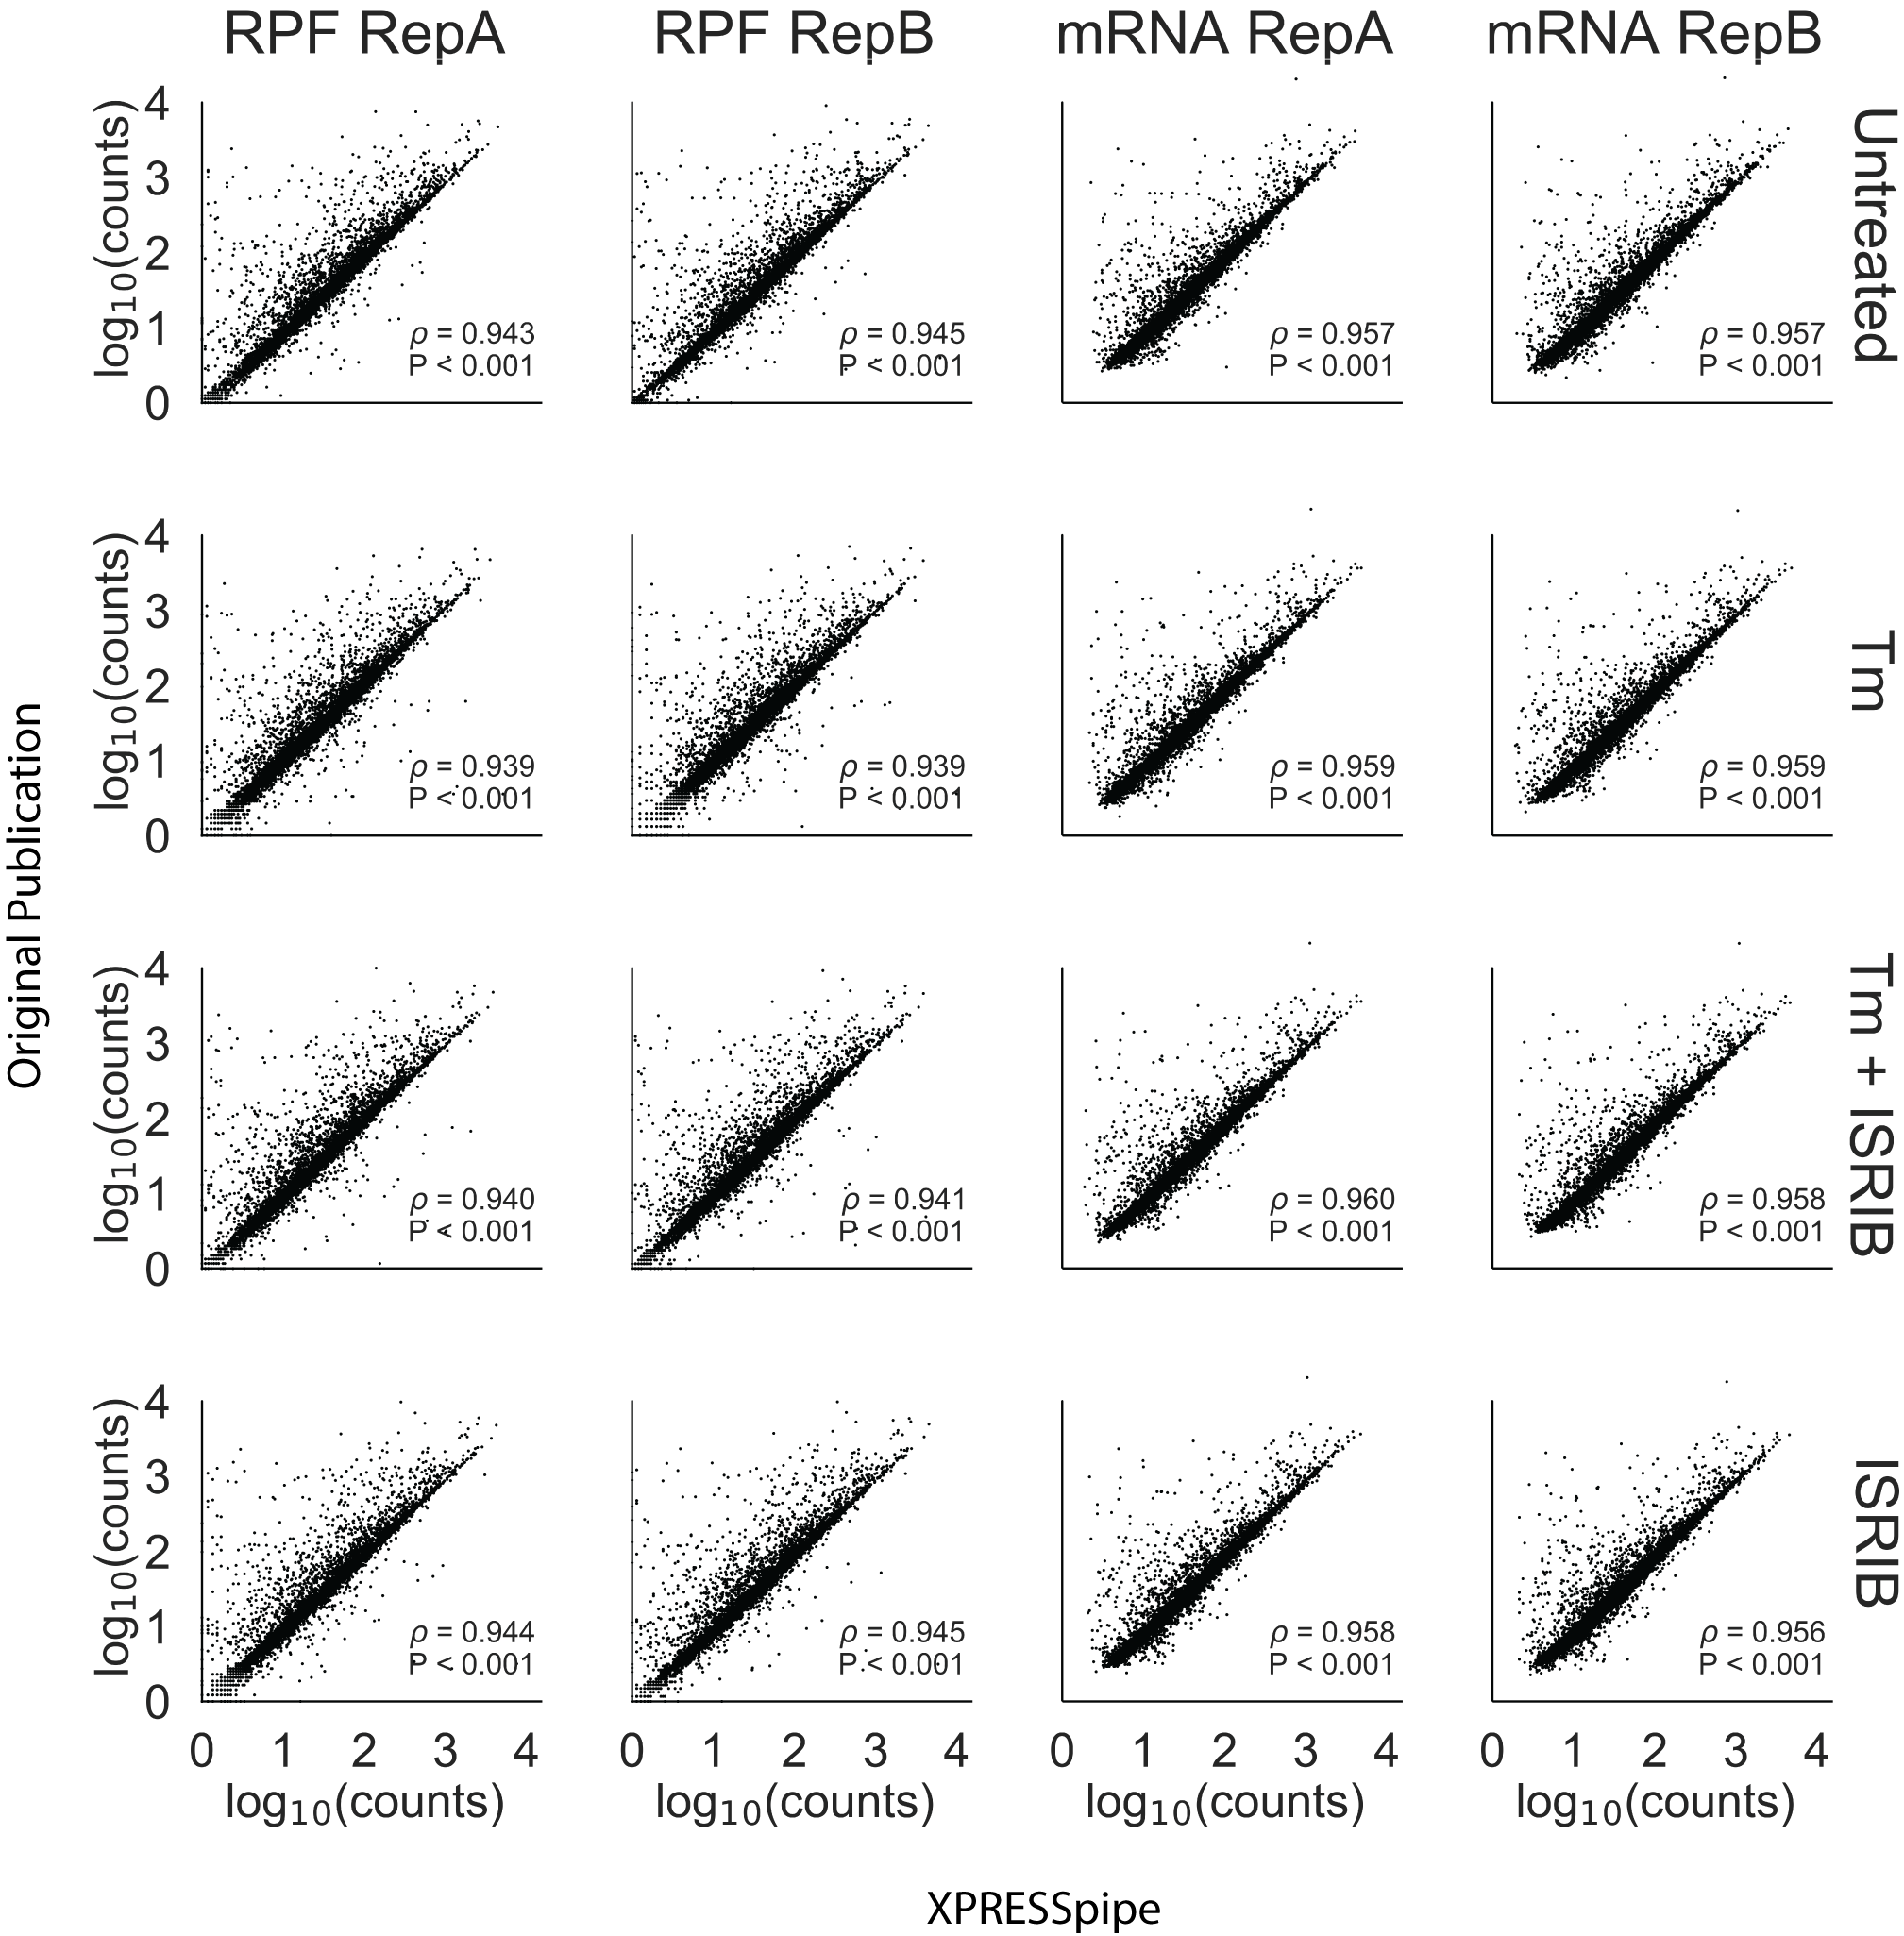
\includegraphics[width=180mm]{figures/xpresspipe_supplement5.png}
  \caption{\textbf{Original ISRIB count data plotted against XPRESSpipe-processed data quantifying with same reference version reveals negligible improvement in comparability between the analytical regimes.} Original samples were processed using Ensembl human build GRCh38 v72, as in the original manuscript, and compared with the original count data provided with the manuscript. XPRESSpipe-prepared counts were thresholded similarly as the original data (each gene needed to have at least 10 counts across all mRNA samples). RepA, biological replicate A. RepB, biological replicate B. RPF, ribosome-protected footprint. Tm, tunicamycin. All $\rho$ values reported are Spearman correlation coefficients.}
  \label{fig:supplement5}
\end{figure}

\begin{figure}
\centering
  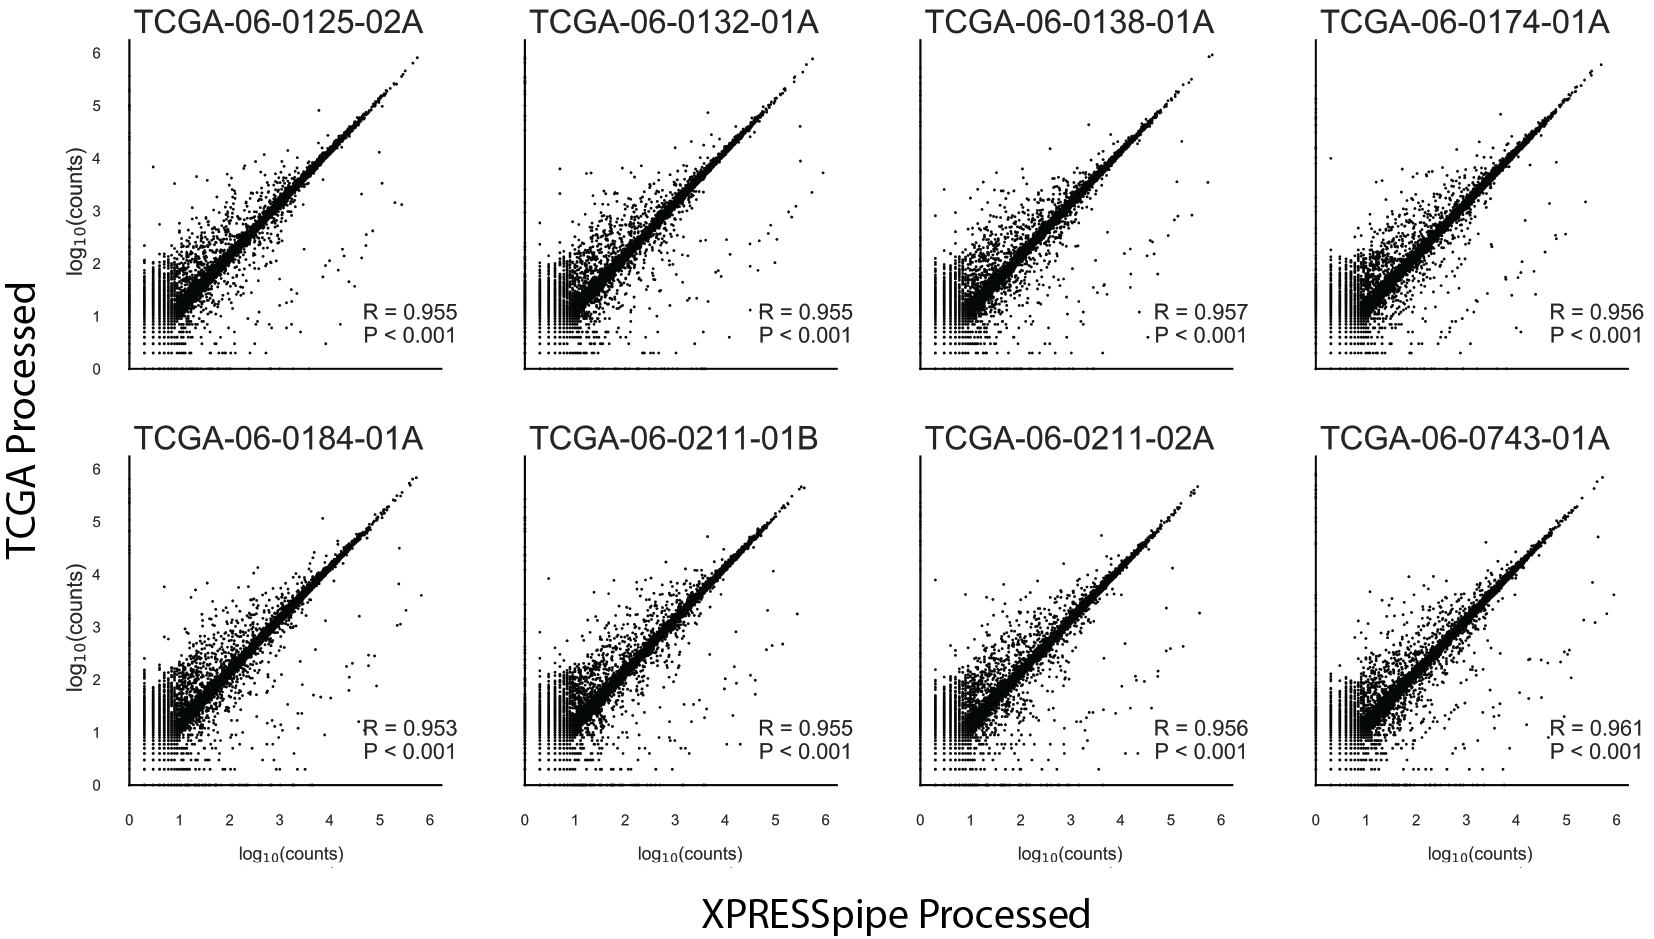
\includegraphics[width=180mm]{figures/xpresspipe_supplement6.png}
  \caption{\textbf{Gene coverage plots for neurologically annotated genes passing strict thresholding.} Coverage plots were generated using XPRESSpipe's geneCoverage module, which collapses introns within the representation.}
  \label{fig:supplement6}
\end{figure}

\begin{figure}
\centering
  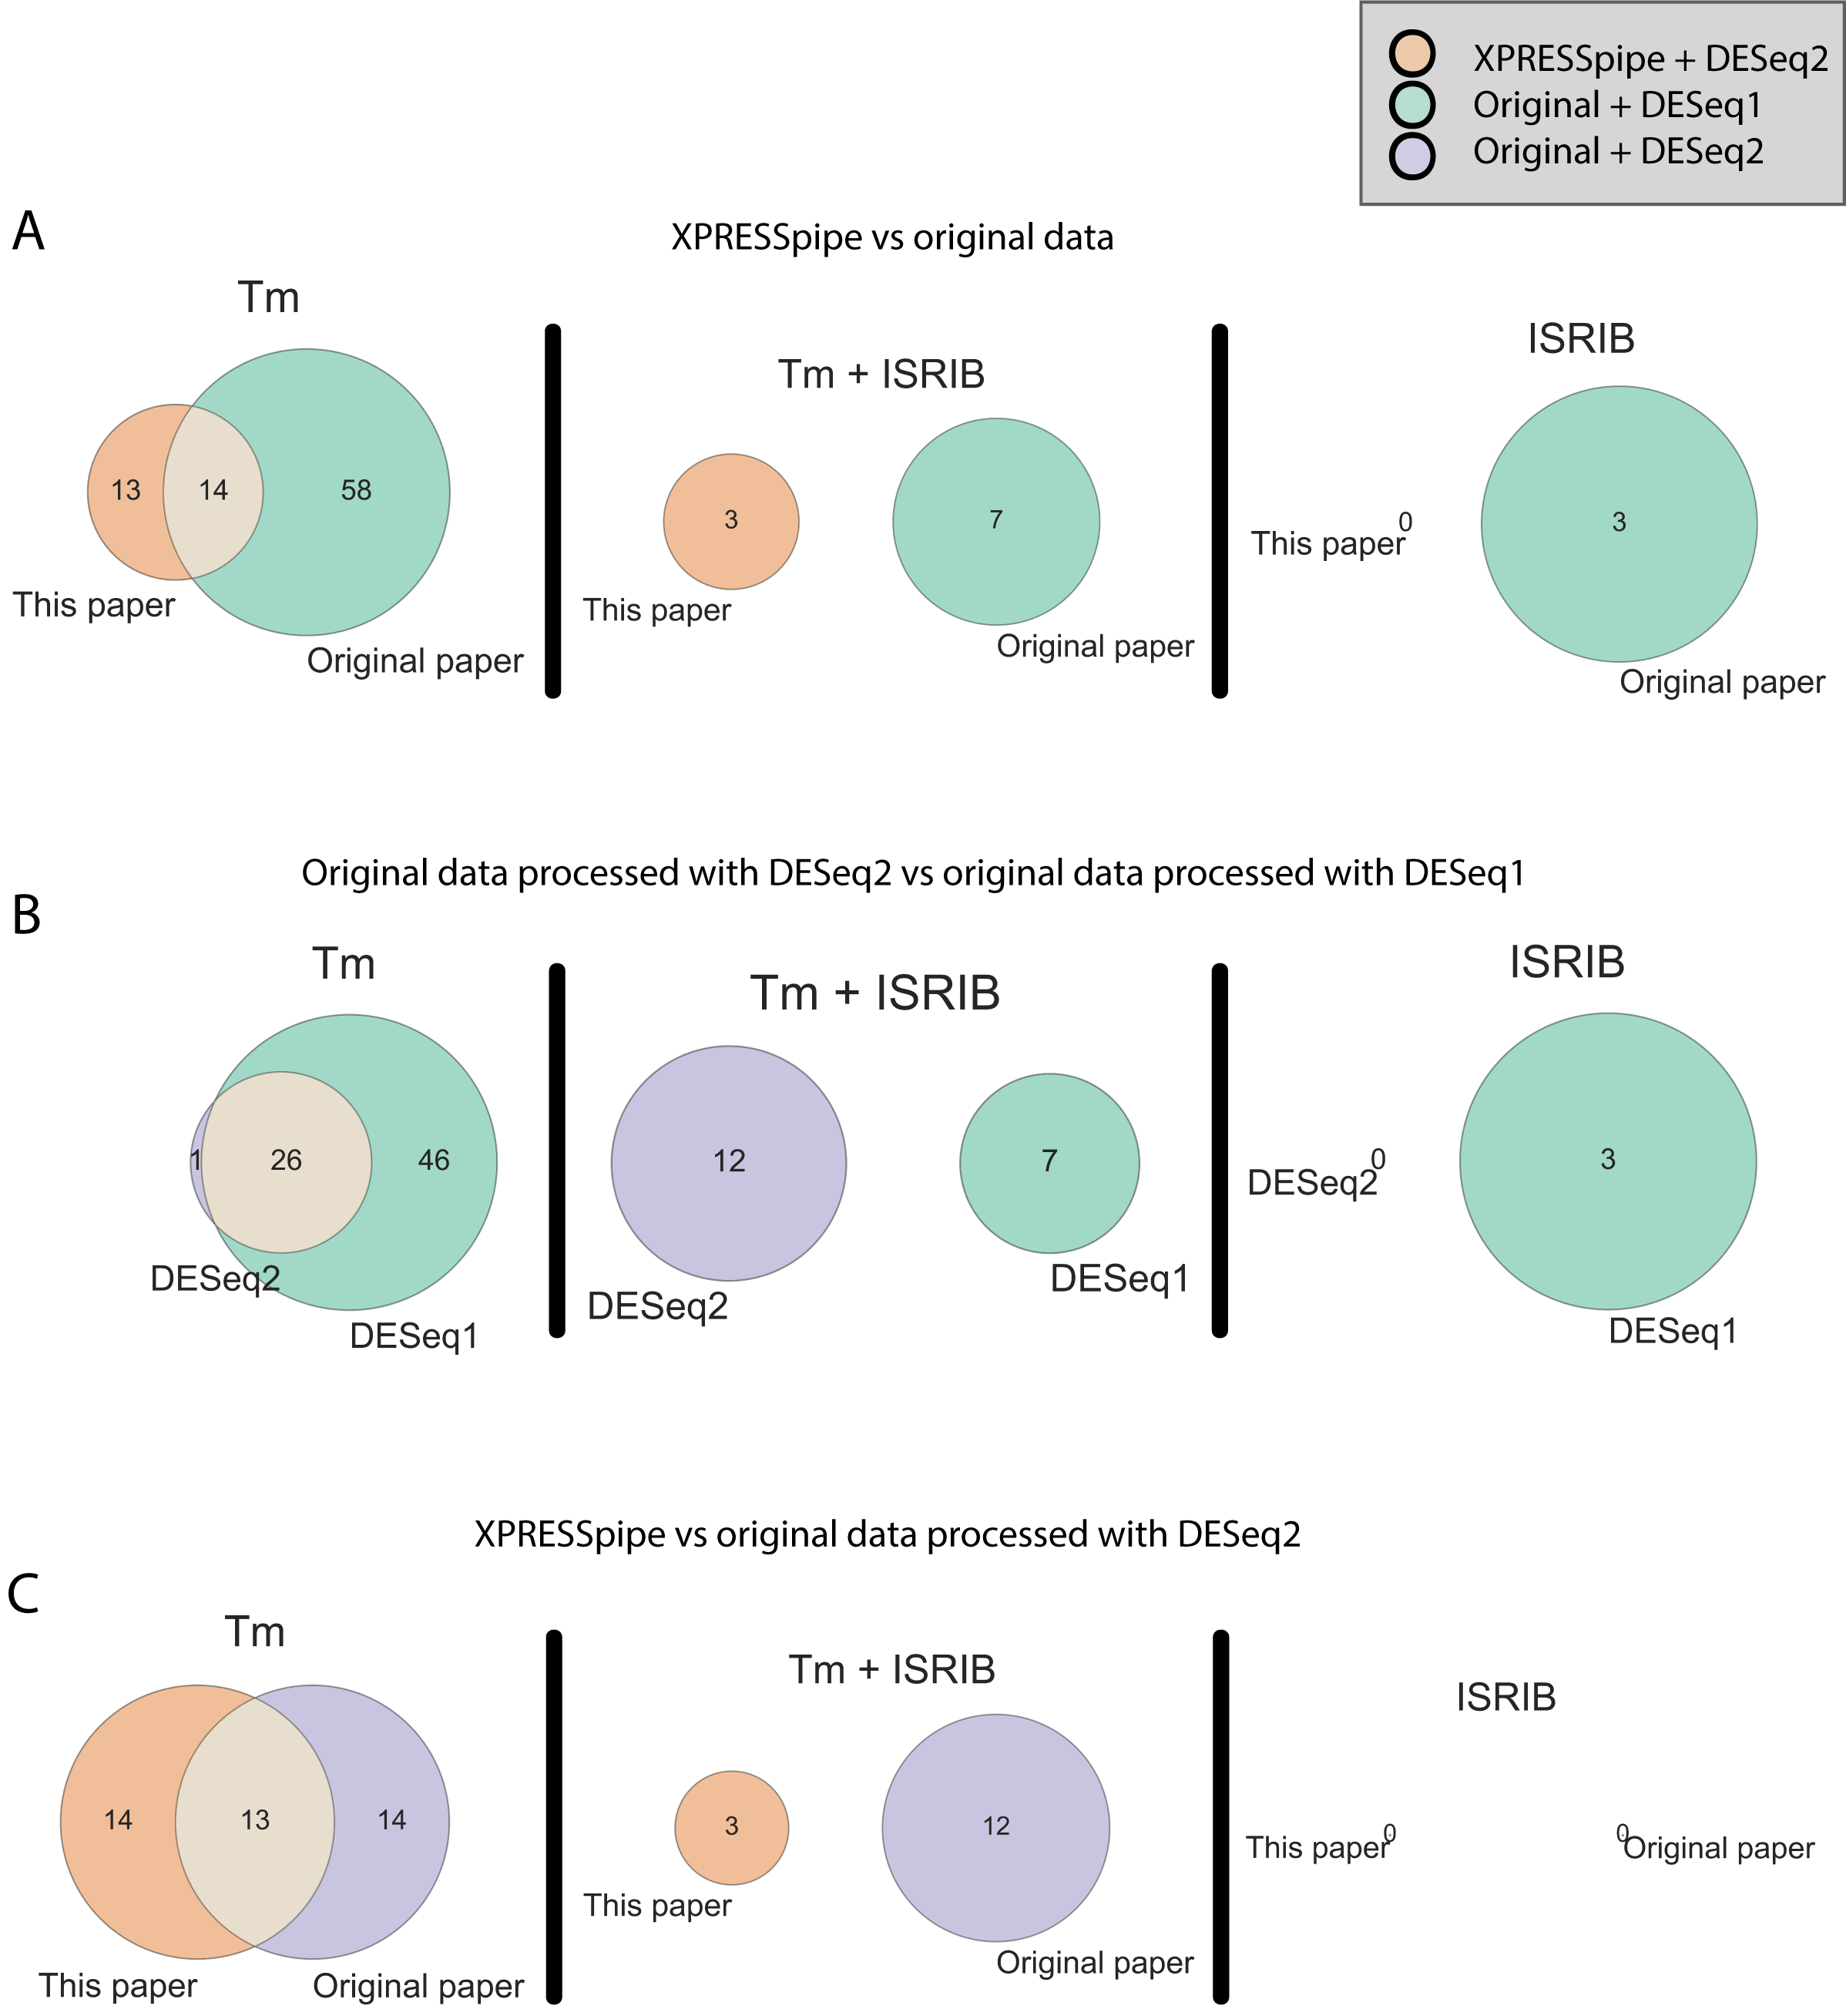
\includegraphics[width=180mm]{figures/xpresspipe_supplement7.png}
  \caption{\textbf{Cross-method analysis comparisons.} A) XPRESSpipe-processed data (orange) versus data as originally presented within original manuscript using original methods (green). B) Comparison of analyses using provided count table in original publication using DESeq2 (purple) versus original analysis provided in manuscript using DESeq1 (green). C) XPRESSpipe-processed (orange) versus originally-processed data (purple), both using DESeq2 for differential expression analysis. Thresholds used were the same as those used in the original study: |log$_2$(Fold Change)| > 1, FDR < 0.1.}
  \label{fig:supplement7}
\end{figure}

\end{document}
